\chapter{Development and evaluation of the AquaCrop weed management procedure}\label{ch:weed}
\chaptermark{Weed management}

This chapter is based on:\\
\longfullcite{vangaelen2016}

\section{Introduction}
Nowadays, studies on agricultural productivity rely increasingly on simulations models. Being more cost- and time-efficient, crop models offer an attractive supplement to field experiments. Crop models are not only used to estimate potential yield levels and investigate causes of yield gaps, but also to evaluate management strategies that can boost crop productivity and water use efficiency. Initially, most crop models were developed to simulate crop production at field scale for historical time series. However, model application has evolved towards large scale studies as well as prediction of future crop productivity.

While most crop models consider yield-limiting factors such as water stress and nutrient deficiencies, biotic factors such as weeds are often neglected. Notwithstanding, considerable yield losses due to weeds are not only faced by smallholder farmers in developing countries \parencite{fao2009}, but also occur in large-scale intensive cropping systems in developed countries \parencite{swanton1993, pimentel2000, milberg2004}. In addition, weeds transpire water and thereby reduce water availability to the crop. This unproductive water consumption is critical in drought-prone regions, where optimizing crop water productivity is a prerequisite for sustainable crop production.

To include the effect of weed infestation in simulation studies, one could apply empirical equations that predict crop yield losses based on variables such as weed density \parencite{cousens1985}, relative time of weed emergence \parencite{cousens1987}, relative leaf area \parencite{kropff1995}, and relative leaf cover of the weeds \parencite{lotz1994}. However, these empirical equations entirely rely on locally calibrated parameters, which hinder extrapolation to other weed species, crop species, locations, environmental conditions, and management practices \parencite{kropff1992b,murphy2002}. Also, process-oriented, mechanistic simulation models such as ALMANAC \parencite{kiniry1992}, APSIM \parencite{keating2003}, CROPSIM \parencite{chikoye1996} and INTERCOM \parencite{kropff1993} have been developed or extended to study crop-weed interactions. However, high requirements for input data, parameter calibration and validation, impede efficient application of these models for a wide range of environmental conditions and cropping systems \parencite{weaver1996}. Particularly in data-scarce regions, application of existing mechanistic simulation models is impractical.

The AquaCrop crop water productivity model \parencite{hsiao2009,steduto2009,raes2009} was developed by the Food and Agriculture Organization of the United Nations (FAO) to estimate yield for herbaceous crops cultivated under various environmental conditions and management practices. Although the model is mechanistic by nature, simulated processes in the crop-soil system are largely simplified. Notwithstanding these simplifications, AquaCrop provides accurate productivity estimates based on a limited number of easily obtainable input variables and parameters. This makes the model practical to apply in data-scarce regions, as well as for studies on a regional scale \parencite{lorite2013, kim2015}. AquaCrop has been applied to assess irrigation and soil fertility management strategies \parencite{geerts2009a, geerts2010,shrestha2013,shrestha2013a,tsegay2015}, but only recently a weed management module was developed for implementation in AquaCrop (test version 5.0). Like the AquaCrop model, this module was developed pursuing an optimal balance between model accuracy, robustness, transparency, and input requirements.

The current study discusses the new AquaCrop calculation algorithms for crop yield simulation in weed-infested fields. Moreover, the performance of the AquaCrop model to simulate the soil water content, canopy cover development and crop production in weed-infested fields is evaluated for two different grain crops grown in various environmental and agronomic conditions. 

\section{Materials and Methods}
\subsection{The AquaCrop model for weed-infested conditions}
AquaCrop simulates crop productivity using a four-step process as discussed in \autoref{ch:aquacrop} \autoref{sec:ch2_ACsteps}. First, green crop canopy cover (\CC) is simulated. In a second step, crop transpiration (\Tr) is simulated considering reference evapotranspiration (\ETo) and the simulated canopy cover. Next, crop transpiration is converted into dry above-ground biomass production (\B). In a final step, crop biomass is converted to crop yield (\Y) by means of the harvest index (\HI). Crop yield per unit of water evapotranspired (\ET) is given by the ET crop water productivity (\WPET). During this four-step simulation process, the model accounts for the effect of various abiotic stresses, including water stress, temperature stress, soil salinity stress and soil fertility stress (\autoref{sec:ch2_abioticfac}). 

When weed stress is considered, AquaCrop directly simulates crop canopy development as it is observed in a weed-infested field (\CCw, \autoref{fig:ch4_CCTheory}). In addition, AquaCrop simulates canopy development of the crop-weed mixture (\CCTOT, \autoref{fig:ch4_CCTheory}), which will be referred to hereafter as `total vegetation'. Simulation of total vegetation canopy cover is crucial since the denser canopy in weed-infested fields affects soil evaporation, transpiration and consequently water availability in the root zone and crop water productivity. In AquaCrop, total vegetation is represented by a theoretical crop with denser canopy cover, but otherwise identical characteristics to the crop growing in a weed-free field (\CCwf). Hence, crop characteristics such as phenology, rooting depth, growing cycle length and sensitivity to abiotic stresses are also applicable to the total vegetation. The denser canopy is reflected by both a higher initial (\CCo) and maximum canopy cover (\CCx). Due to this denser canopy and assumption of equal growing cycle length,  the canopy decline rate of the total vegetation is also higher compared to the decline rate of the crop. 
 
\begin{figure}[tbhp]
	\centering
		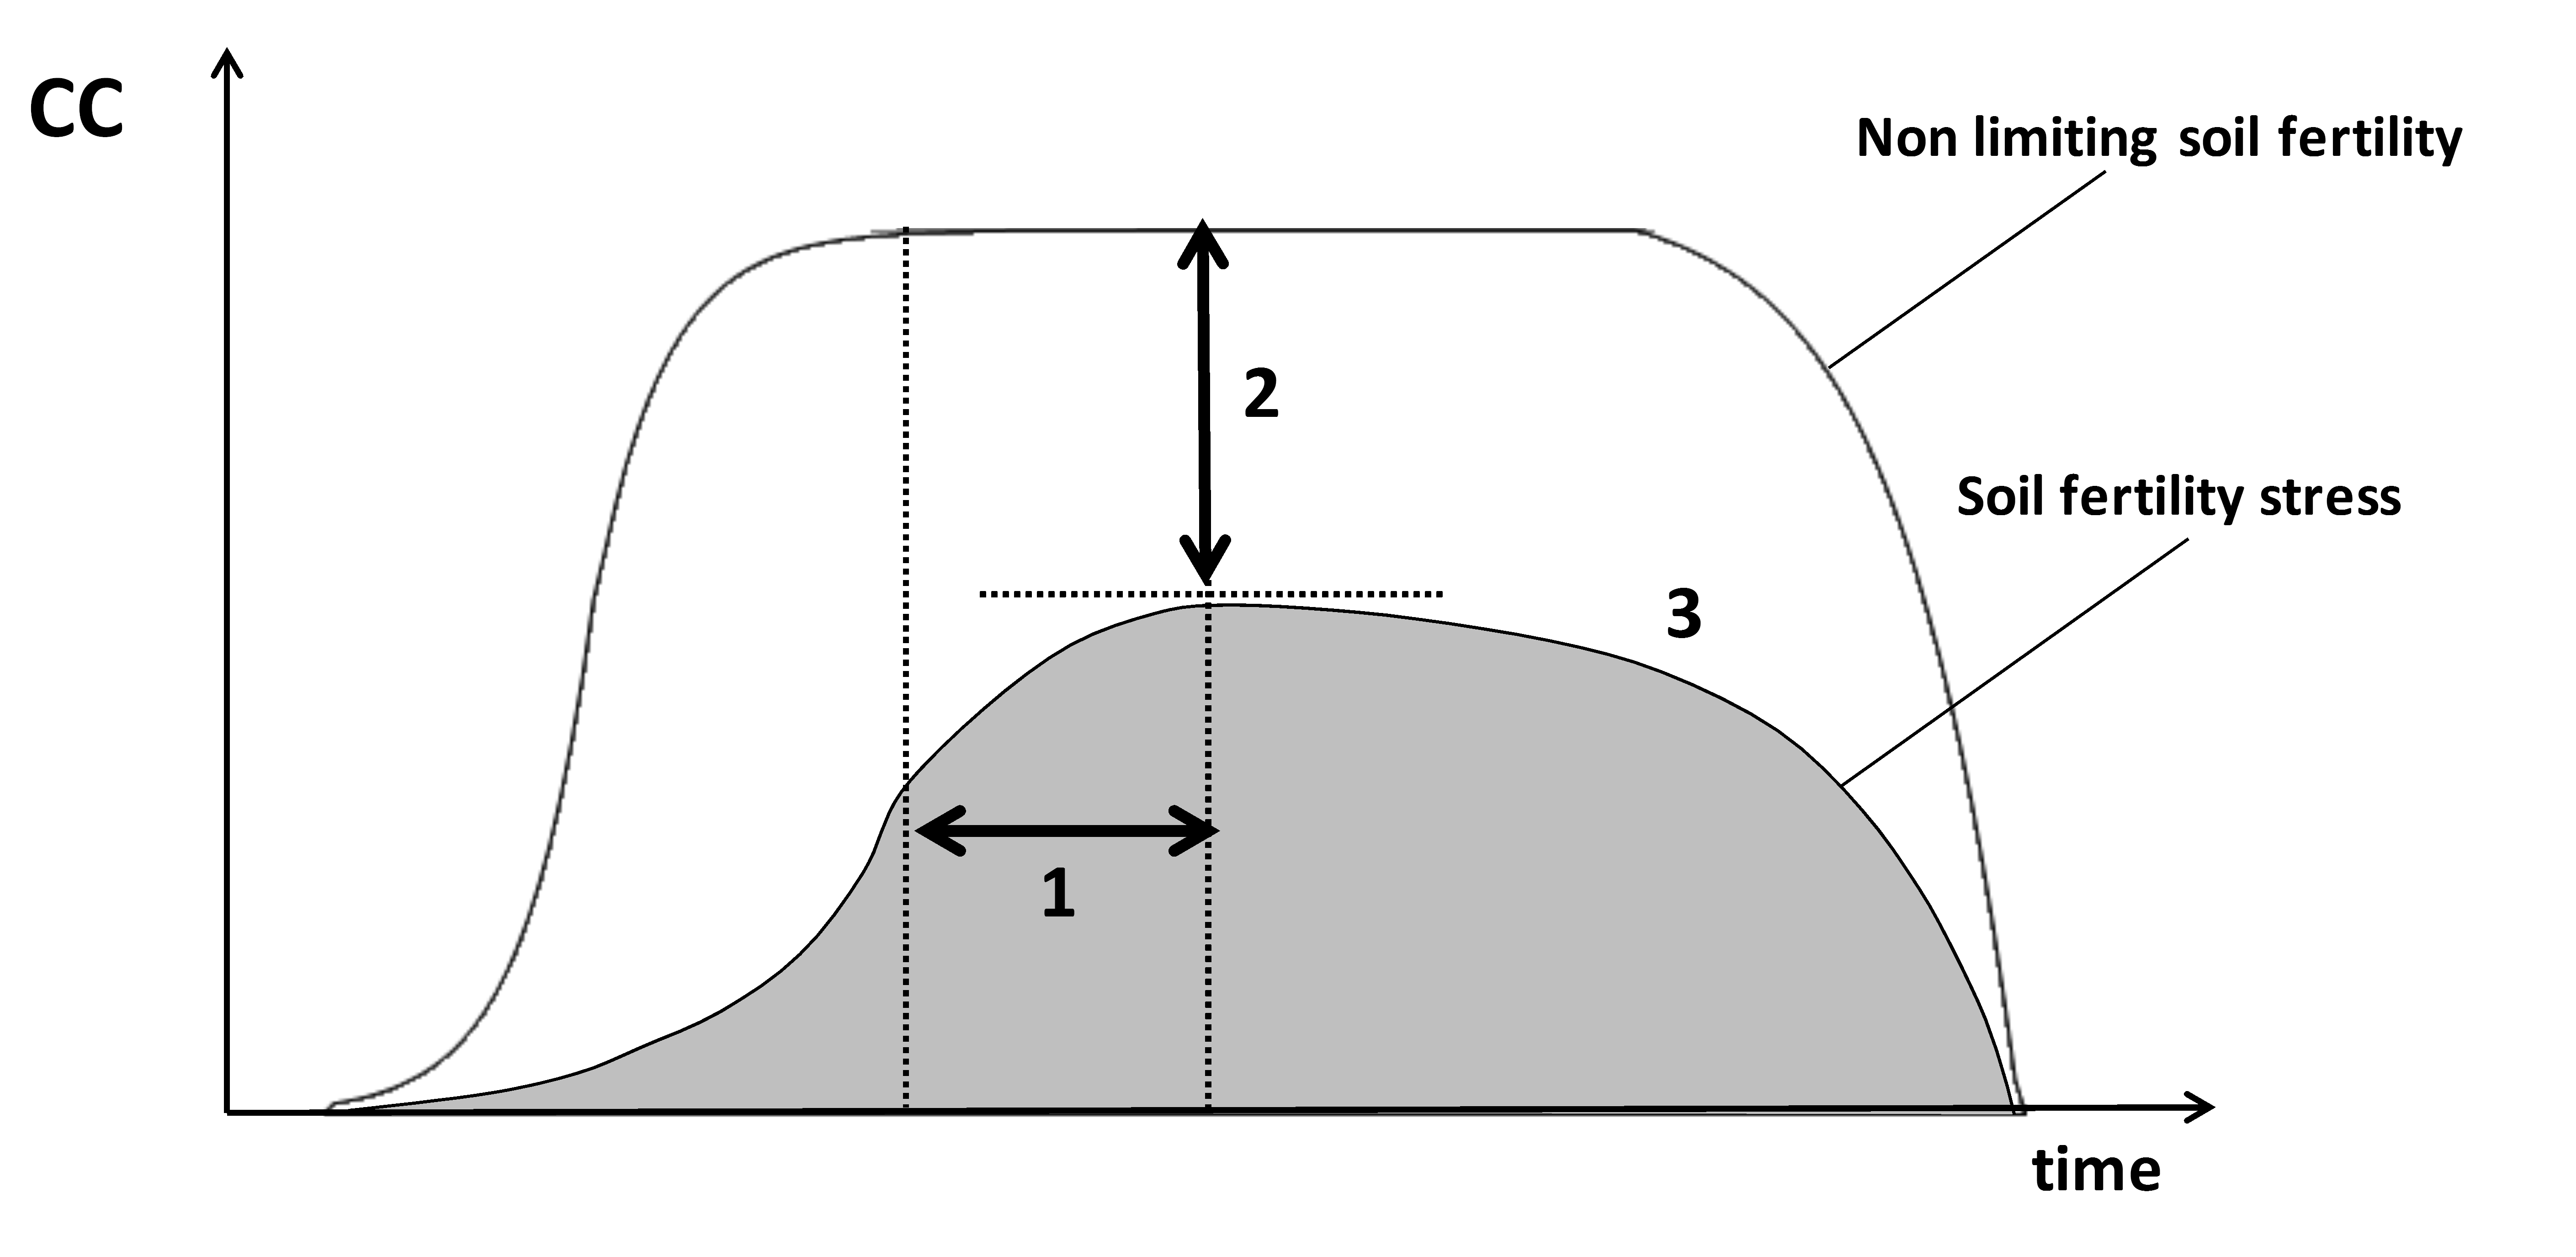
\includegraphics[width=10cm]{CCTheory_600dpi.png}
	\caption{Weed infestation affects the simulated (1) initial canopy cover, (2) maximum canopy cover, and (3) canopy decline rate. As weeds take up empty space or suppress the crop, the crop canopy cover in weed-infested conditions (\CCw) is lower compared to weed-free conditions (\CCwf). Moreover, the canopy cover of the total vegetation (\CCTOT) is higher and has a faster decline compared to the crop canopy cover in weed-free conditions (\CCwf).}
	\label{fig:ch4_CCTheory}
\end{figure}
 
Simulation of both the total vegetation and crop canopy cover in weed-infested fields is completely determined by two user-specified inputs: (i) the weed infestation level or amount of weeds and (ii) the weed-induced increase of total canopy cover. 

The weed infestation level is quantified by means of the relative leaf cover of weeds (\RC, \autoref{eq:ch4_RC}) as defined by \textcite{lotz1994}. 
\begin{equation}
 RC=\dfrac{WC}{CC_{TOT}}=\dfrac{WC}{WC+CC_{W}}
  \label{eq:ch4_RC}
\end{equation}
where \RC is the relative leaf cover of weeds (\si{m^2/m^2}), $WC$ is the area covered by weeds per unit ground area (\si{m^2/m^2}), \CCw is the area covered by the crop per unit ground area in a weed-infested field (\si{m^2/m^2}), and \CCTOT is the area covered by the total vegetation (crop-weed mixture) per unit ground area (\si{m^2/m^2}). 

Relative weed cover is a multi-species canopy characteristic that varies during the growing season. Since the weed's share in leaf area at time of canopy closure is regarded as a good indicator of crop-weed competition \parencite{kropff1991}, AquaCrop requires input of \RC observed at the time maximum crop canopy cover is reached. 

The weed-induced increase of total canopy cover (\fweed) is defined by \autoref{eq:ch4_fweed}: 
\begin{equation}
 f_{weed}=\dfrac{CC_{x,TOT}}{CC_{x,WF}}
  \label{eq:ch4_fweed}
\end{equation}
where \fweed is the weed-induced increase of total canopy cover (-), $CC_{x,TOT}$ is the maximum total vegetation canopy cover (\si{m2/m^2}) and $CC_{x,WF}$ is the maximum crop canopy cover in weed-free conditions (\si{m2/m^2}). 

A large \fweed value indicates that weeds predominantly fill any empty gaps in the crop canopy cover, which results in a strong increase of the total canopy cover. A small \fweed value, on the other hand, indicates that weeds predominantly suppress crop growth by `stealing' light. This results in a small increase in total canopy cover. Hence, for a certain weed infestation level (\RC), differences in weed competitive abilities can result in different total vegetation canopy covers, and consequently different \fweed values. The AquaCrop user defines \fweed either directly or by specifying $CC_{x,TOT}$ for the selected weed infestation level and optimal growing conditions (no fertility, water or salinity stress). In addition, AquaCrop can automatically determine \fweed based on a user-specified canopy expansion factor (\fshape). This \fshape factor fixes the relation between the observed weed infestation level (\RC) and the maximum total vegetation canopy cover ($CC_{x,TOT}$) for optimal growing conditions (\autoref{fig:ch4_fshape}), and consequently represents the competitive ability of weeds to compete with the crop for light.
 
\begin{figure}[tbhp]
	\centering
		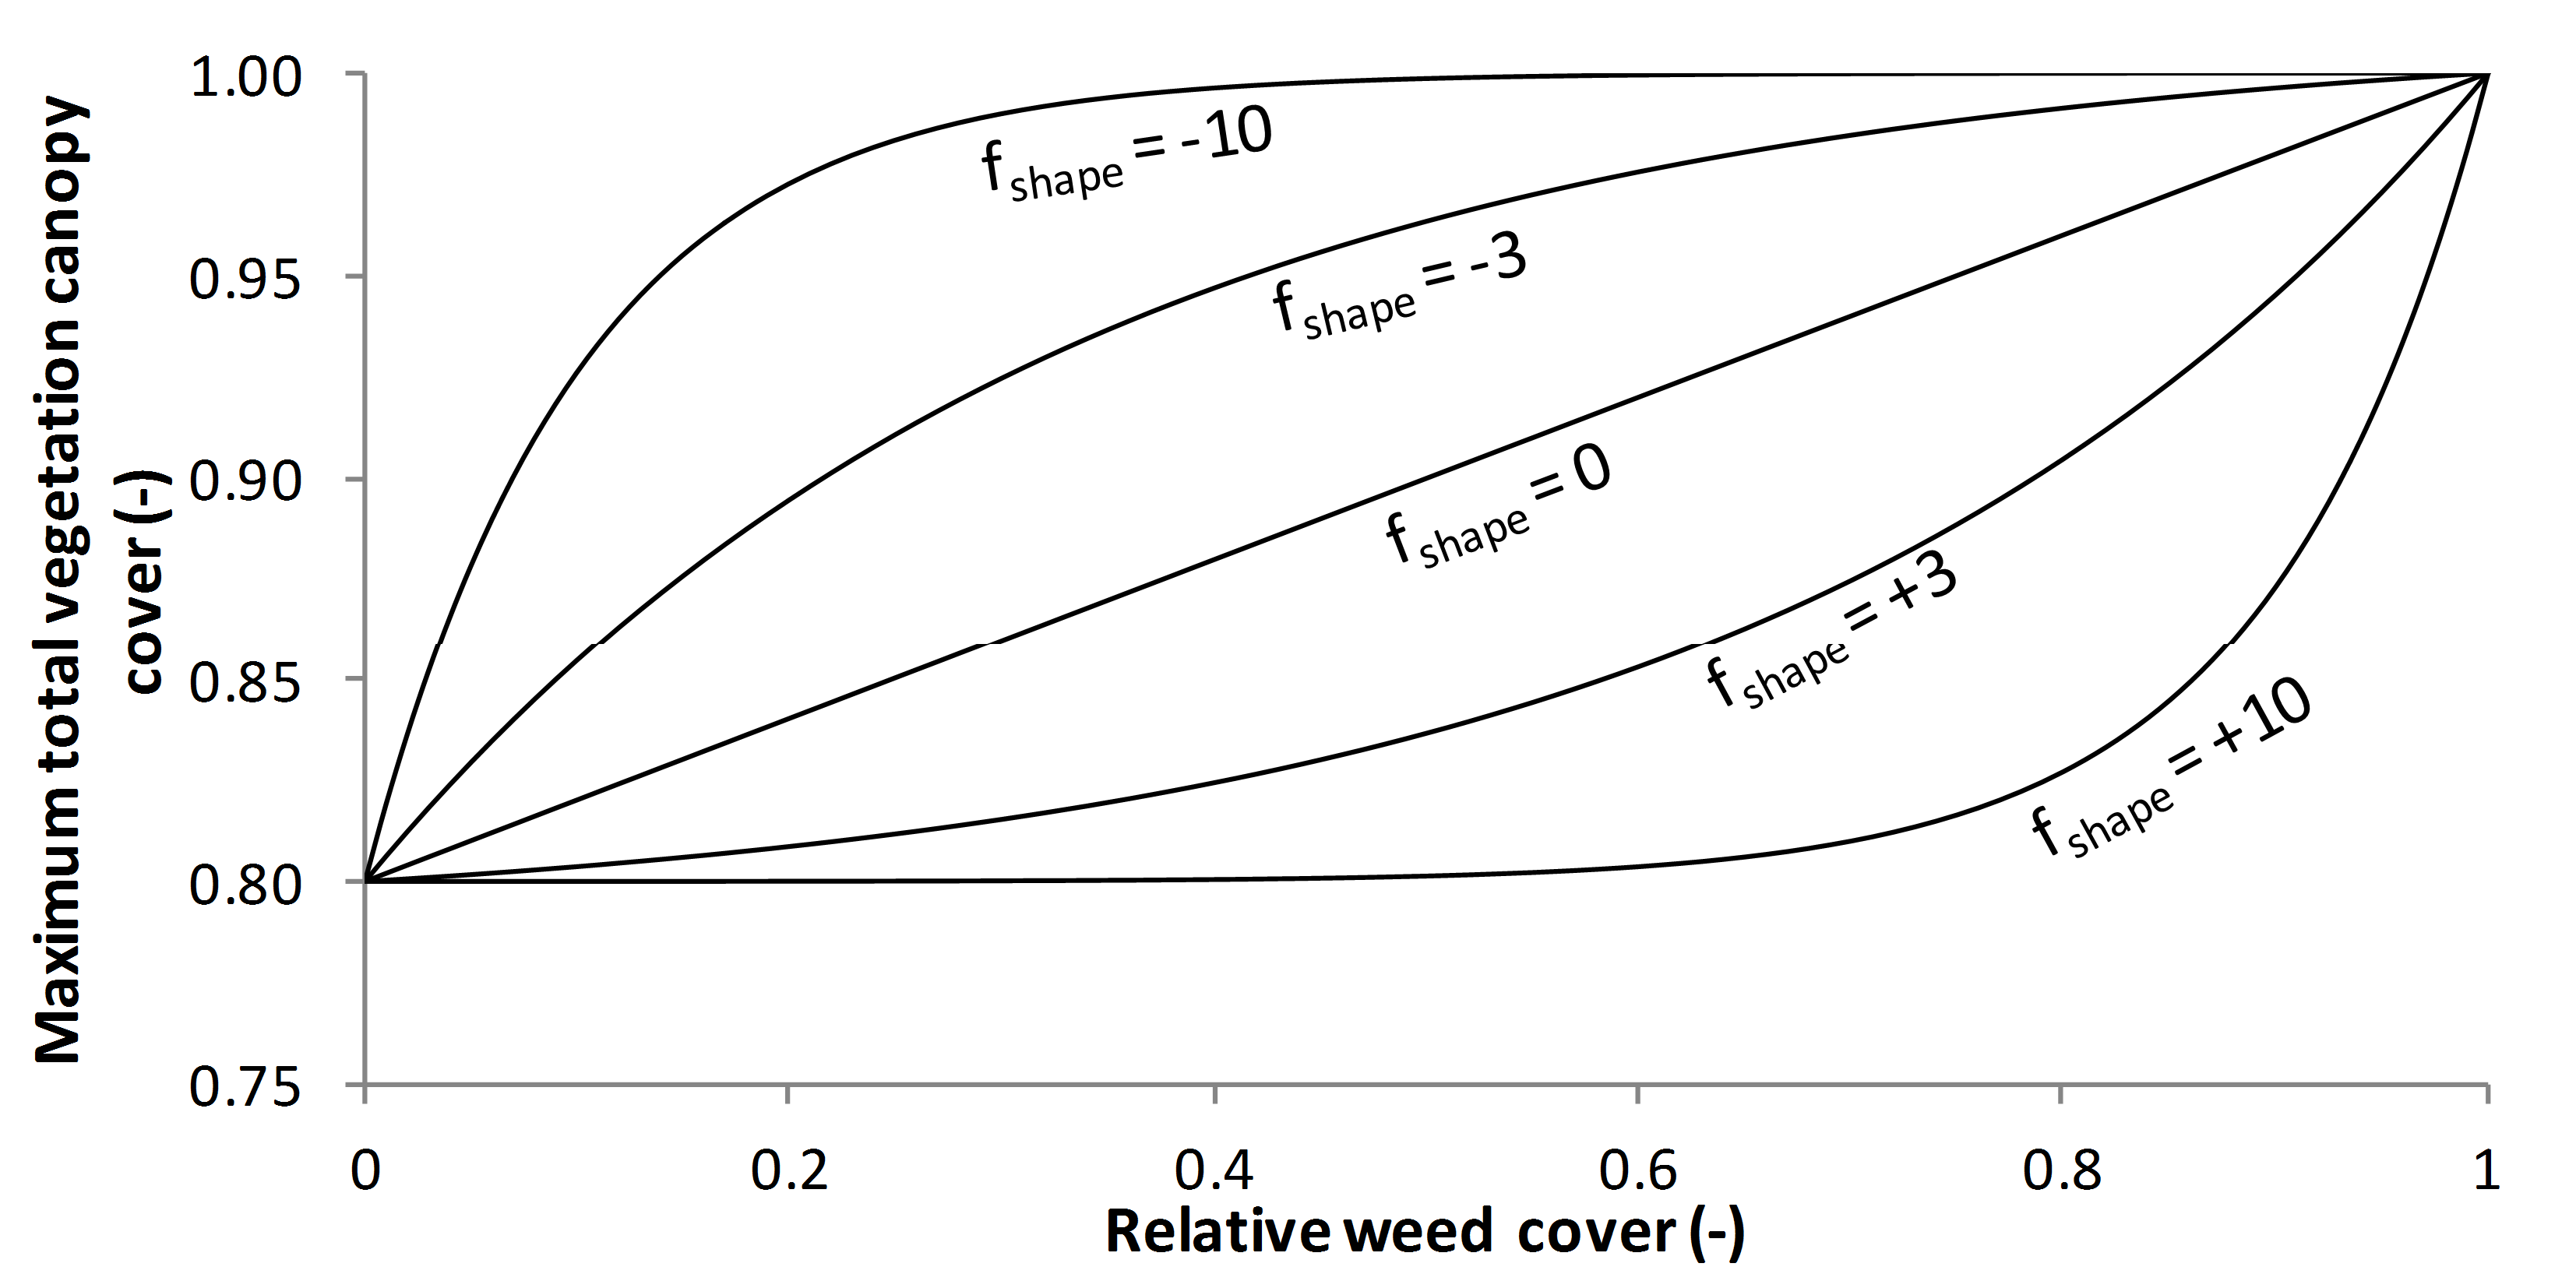
\includegraphics[width=10cm]{fshape_600dpi.png}
	\caption{Relationship between maximum total vegetation canopy cover ($CC_{x,TOT}$) and relative cover of weeds (\RC) is determined by the canopy expansion factor (\fshape). This example presents a crop with a maximum canopy cover ($CC_{x,WF}$) of 0.8 in weed-free conditions.}
	\label{fig:ch4_fshape}
\end{figure} 
 

An AquaCrop simulation for weed-infested conditions starts by simulating total vegetation canopy cover (\CCTOT) by multiplying the crop canopy cover under weed-free conditions ($CC_{x,WF}$) with \fweed. Next, \CCTOT is corrected for water, soil fertility or soil salinity stress using the stress thresholds calibrated for the crop. Thereby it is assumed that weeds are equally as sensitive to those stresses than the crop. Subsequently, the crop canopy cover for weed-infested conditions (\CCw) is derived from \CCTOT based on \RC (\autoref{eq:ch4_RC}). Finally, simulation of \CCw enables simulation of crop transpiration, crop biomass, crop yield and crop water productivity in weed-infested fields using the standard AquaCrop procedure (\autoref{eq:ch2_Tr} to \autoref*{eq:ch2_WPET}). 

Since weeds take up water and affect the soil water balance, AquaCrop calculates the soil water content in the root zone of a weed-infested field considering the total vegetation canopy cover. Evaporation and transpiration of the total vegetation are simulated considering the denser canopy of weed-infested versus weed-free fields (\CCTOT versus \CCwf). The simulated soil water content is used to correct the simulated crop and total vegetation canopy cover, crop transpiration and yield formation in a weed-infested field for water stress. It should be noted that increased water stress is the only mechanism through which weeds affect the harvest index in AquaCrop. An additional adjustment to the harvest index for weeds is not considered. Furthermore, weeds increase nutrient stress by `stealing' crop nutrients. For that reason, the soil fertility level is adapted during simulation. In addition, a weed-induced increase of total canopy cover is no longer considered (\fweed is 1), since low soil fertility restricts total canopy cover development to the level that can be reached in weed-free conditions ($CC_{x,TOT}$ equals $CC_{x,WF}$).

\subsection{Field experiments}
The AquaCrop weed management algorithms were tested against two sets of experimental data (\autoref{tab:ch4_metExp}). The first set comprised data of four experiments conducted with barley (\textit{Hordeum vulgare} L.) in the drought-prone, degraded highlands of Tigray in northern Ethiopia. The second set consisted of data from a field experiment with wheat (\textit{Triticum aestivum} L.) conducted in semi-arid Wagga Wagga, Australia. 

All experiments were setup with a split-plot design in which water treatment was the main factor and the weed treatment the sub-factor (\autoref{tab:ch4_metExp}). In S1 water treatments, crop development or production were affected by water stress, while crops did not suffer water stress in S0 treatments. Occurrence of water stress was caused by insufficient rainfall, inadequate irrigation, or the presence of a rainshelter. Since observed differences between water treatments were not significant for barley in all four experiments \parencite{abrha2013}, only one water treatment was retained for the current study (\autoref{tab:ch4_metExp}). In Dejen and Maiquiha, naturally occurring weeds were retained and weed treatments consisted of different hand weeding frequencies: no weeding, one time weeding at 21 days after emergence (only in 2009) and frequent weeding (at least three times). The majority of weed species were broad-leaved (e.g. \textit{Scorpiurus muricatus}), but grasses (e.g. \textit{Avena} sp., \textit{Digitaria} sp.) and sedges (e.g. \textit{Cyperus} sp.) were also present.  In Mekelle, wild oat (\textit{Avena fatua} L.) was sown together with barley at a proportion of  0\%, 5\%, 20\% and 50\% of the total amount of seeds. In Wagga Wagga, ryegrass (\textit{Lolium rigidum} Gaud.) was sown aiming at a weed density of 250 plants/m2. At all experimental sites, the plots were kept free from pests, diseases and undesired weeds throughout the growing season. Moreover, all plots were kept at optimal fertility to ensure that neither crops nor weeds would suffer from nutrient stress. During the growing season observations of local daily weather, soil characteristics, irrigation and soil fertility management, soil water content, crop phenology, crop and weed canopy (leaf area index (LAI) or green canopy cover), dry above-ground crop biomass and crop yield, were recorded. Observations of the second data set were retrieved from the paper by \textcite{deen2003} or shared by those authors. Unfortunately, not all data could be retrieved; some observations of the weed-infested plots were missing (e.g. yield and soil water content) or observations were limited to average values without records of the deviation between replications. More detailed information on the experimental set-up and data collection is described by \textcite{deen2003} for wheat, and \textcite{abrha2012} and \textcite{abrha2013} for barley.  

\begin{landscape}
\begin{table}[htbp]
  	\caption{Experimental sites, setup and environmental conditions of the five experiments. Water treatments consist of absence (S0) or presence (S1) of water stress. Seasonal aridity indices represent the ratio of total rainfall to reference evapotranspiration (\ETo) during the growing season.}
    \resizebox{\linewidth}{!}
		{
	\begin{threeparttable}
  	\centering
		\begin{tabular}{lcrrcc}
	\toprule
\textbf{} & \multicolumn{4}{c}{\textbf{Dataset 1}} & \textbf{Dataset 2} \\
\textbf{Experimental site} & Dejen & \multicolumn{1}{c}{Dejen} & \multicolumn{1}{c}{Maiquiha} & Mekelle & Wagga Wagga \\
\midrule
Country & Ethiopia & \multicolumn{1}{c}{Ethiopia} & \multicolumn{1}{c}{Ethiopia} & Ethiopia & Australia \\
Coordinates & 13°20' N, 39°22' E & \multicolumn{1}{c}{13°20' N, 39°22' E} & \multicolumn{1}{c}{13°48'N, 39°27'E} & 13°28' N, 39°29' E & 35°10' S, 147°28' E \\
Altitude (m a.s.l.) & 2128  & \multicolumn{1}{c}{2128} & \multicolumn{1}{c}{2078} & 2212  & 200 \\
\midrule
\textbf{Experimental setup} &       &       &       &       &  \\
Location & Farmer training centre & \multicolumn{1}{c}{Farmer's field} & \multicolumn{1}{c}{Farmer's field} & Research station & Research station \\
Season & 2009  & \multicolumn{1}{c}{2010} & \multicolumn{1}{c}{2009} & 2010  & 1998 \\
Sowing date & 10/07/2009 & \multicolumn{1}{c}{13/07/2010} & \multicolumn{1}{c}{15/07/2009} & 15/07/2010 & 18/05/1998 \\
Replications & 3     & \multicolumn{1}{c}{3} & \multicolumn{1}{c}{3} & 3     & 5 \\
Crop  & Barley & \multicolumn{1}{c}{Barley} & \multicolumn{1}{c}{Barley} & Barley & Wheat \\
Weed species & Natural mix & \multicolumn{1}{c}{Natural mix} & \multicolumn{1}{c}{Natural mix} & Wild oat & Ryegrass \\
Water treatment(s) & S0    & \multicolumn{1}{c}{S0} & \multicolumn{1}{c}{S1} & S0    & S0,S1 \\
\multirow{2}[1]{*}{Weed treatments} & Hand weeding frequency: & \multicolumn{1}{c}{Hand weeding frequency:} & \multicolumn{1}{c}{Hand weeding frequency:} & Weed seed proportion: & Weed density: \\
      & 0, 1, $\geq$3 times/season & \multicolumn{1}{c}{0, $\geq$3 times/season} & \multicolumn{1}{c}{0, 1, $\geq$3  times/season} & 0, 5, 20, 50\% & 0, 250 \si{plants/m^2} \\
\midrule
\textbf{Environmental conditions} &       &       &       &       &  \\
Soil type & Luvisol & \multicolumn{1}{c}{Luvisol} & \multicolumn{1}{c}{Leptosol} & Cambisol & Red-brown earth soil \\
Soil texture & Sandy loam to silt loam & \multicolumn{1}{c}{Loam to silt loam} & \multicolumn{1}{c}{Silt loam} & Sandy (clay) loam & Loam, silty clay \\
Seasonal rainfall (mm) & 301   & \multicolumn{1}{c}{443} & \multicolumn{1}{c}{239} & 552   & 420 (S0) and 122 (S1)$^\ast$ \\
Seasonal \ETo (mm) & 324   & \multicolumn{1}{c}{280} & \multicolumn{1}{c}{367} & 285   & 353 \\
Seasonal aridity index (-) & 0.93  & \multicolumn{1}{c}{1.58} & \multicolumn{1}{c}{0.65} & 1.94  & 1.19 (S0) and 0.35 (S1)$^\ast$ \\
\bottomrule
    	\end{tabular}%  
    	\begin{tablenotes}
      	\item[$\ast$] Seasonal rainfall was affected by the presence of a rain shelter in the S1 treatment.	 
    	\end{tablenotes}  	
        \end{threeparttable}
        }
  \label{tab:ch4_metExp}%
\end{table}%
\end{landscape}

\subsection{Model input} 
Observations of local climatic data, irrigation practices, soil characteristics and initial soil water content were used as inputs in a test version of AquaCrop 5.0. Simulations were conducted assuming non limiting soil fertility for all plots. Default crop parameters were used as a starting point; thereafter non-conservative crop parameters were adjusted to match the characteristics of the local cultivar and environment (\autoref{tab:ch4_croppar}). Crop developments stages were specified in growing degree days (GDD) to enable temperature dependent crop canopy development. Conservative crop parameters, which by definition are independent of cultivar, management and geographical location, were kept default, except for wheat. Since AquaCrop does not consider typical processes for winter crops such as vernalization, dormancy and cold acclimation, simulation of winter wheat development required adaptation of some conservative crop parameters (\autoref{tab:ch4_croppar}) following the example of \textcite{vanuytrecht2013}.

\begin{table}[htbp]
\begin{tabularx}{\textwidth}{Xcccc}
  	\caption{Key crop parameters for barley and wheat grown at the experimental sites. Values that were changed from the default are presented in bold. * indicates the values for Mekelle.}\\
\toprule
& & & \textbf{Barley} & \textbf{Wheat} \\
\midrule
\multicolumn{3}{l}{\textbf{Non-conservative parameters}}        &       &  \\
Initial canopy cover &\CCo & \%    & 2.70/\textbf{2.96$^\ast$} & \textbf{1.95} \\
Maximum canopy cover &\CCx & \%    & 80/\textbf{88$^\ast$} & \textbf{88} \\
Time to emergence &eme & GDD   & 98    & \textbf{80} \\
Time to start senescence &sen & GDD   & 924   & \textbf{710} \\
Total length of crop cycle & mat & GDD   & 1296  & \textbf{1401} \\
Maximum effective rooting depth &rtx & m     & 1.3   & \textbf{1.2} \\
\textbf{} &       &       &  \\
\midrule
\multicolumn{3}{l}{\textbf{Conservative parameters}}        &       &  \\
Canopy growth coefficient & cgc & \%/GDD & 0.9 & \textbf{1.115} \\
Canopy decline coefficient &cdc & \%/GDD & 0.6 & 0.400 \\
Base temperature &tb & \si{\degreeCelsius}    & 2     & \textbf{4} \\
Upper temperature &tup & \si{\degreeCelsius}    & 28    & 26 \\
Minimum growing degrees required for full biomass production & stbio & \si{\degreeCelsius/d} & 14    & \textbf{10} \\
Normalized biomass water productivity & \WPster & \si{g/m^2}  & 15.0    & \textbf{18.5} \\
Reference harvest index & hio  & \%    & 33    & 48 \\
\bottomrule
\end{tabularx}%
  \label{tab:ch4_croppar}%
\end{table}%

Weed management inputs (\RC and \fweed), listed in \autoref{tab:ch4_weedpar}, were determined applying  \autoref{eq:ch4_RC} and \ref{eq:ch4_fweed} to available \CCwf, \CCw and $WC$ observations of well-watered plots at time of maximum crop canopy cover. For wheat experiments, LAI values were first converted to CC values using \autoref{eq:ch4_LAIconvert} \parencite{kropff1993} with a light extinction coefficient (l) of 0.6 and 0.5 for wheat and ryegrass respectively \parencite{lantinga1999,acevedo2002}.
\begin{equation}
 CC=1-exp\left(\sum_{i=1}^n l_i \cdot LAI_i \right) 
  \label{eq:ch4_LAIconvert}
\end{equation}
where CC is the green canopy cover (\si{m^2/m^2}), $l_i$ is the light extinction coefficient (-), and $LAI_i$ the leaf area index (\si{m^2/m^2}) of species i as observed in a field with n species.

Since weed species were similar for all weed treatments of the same experiment, a single canopy expansion factor (\fshape) was selected for all treatments. The \fshape value was selected so that the resulting \fweed values, automatically determined by AquaCrop, approached the observed \fweed values well. Moreover, water availability in wheat plots affected the amount of weeds at time of canopy closure so that different \RC values were selected for both water treatments. 
\begin{table}[htbp]
  	\caption{Weed treatments with selected AquaCrop weed management input: relative weed cover (\RC) and weed-induced total canopy cover increase (\fweed) with corresponding canopy expansion factor (\fshape). Water treatments consist of absence (S0) or presence (S1) of water stress.}
    \resizebox{\textwidth}{!}
		{
\begin{tabular}{lccccc}
\toprule
\textbf{Experiment} & \textbf{Water} & \textbf{Weed} & \textbf{\RC} & \textbf{\fshape} & \textbf{\fweed} \\
 & \textbf{treatment} & \textbf{treatment} & \textbf{(\%)} & \textbf{(-)} & \textbf{(-)} \\
\midrule
Dejen, 2009 & S0    & Weeding frequency&       &       &  \\
      &       & $\geq$3 /season    & 0     & -     & - \\
      &       & 1 /season     & 15    & 1     & 1.02 \\
      &       & 0 /season     & 50    & 1     & 1.10 \\
\midrule
Dejen, 2010 & S0    & Weeding frequency &       &       &  \\
      &       & $\geq$3 /season   & 0     & -     & - \\
      &       & 0 /season    & 13    & -5.5  & 1.13 \\
\midrule
Maiquiha, 2009 & S1    & Weeding frequency &       &       &  \\
      &       & $\geq$3 /season   & 0     & -     & - \\
      &       & 1 /season     & 14    & -1    & 1.05 \\
      &       & 0 /season    & 30    & -1    & 1.10 \\
\midrule
Mekelle, 2010 & S0    & Weed seed proportion &       &       &  \\
      &       & 0\%   & 0     & -     & - \\
      &       & 5\%   & 8     & 10    & 1.00 \\
      &       & 20\%  & 23    & 10    & 1.00 \\
      &       & 50\%  & 49    & 10    & 1.00 \\
\midrule
Wagga Wagga, 1998 & S0    & Weed density  &       &       &  \\
      &       & 0 \si{plants/m^2}    & 0     & -     & - \\
      &       & 250 \si{plants/m^2}  & 20    & -10   & 1.12 \\
      & S1    & 0 \si{plants/m^2}    & 0     & -     & - \\
      &       & 250 \si{plants/m^2}  & 15    & -10   & 1.11 \\
\bottomrule
\end{tabular}%
}
  \label{tab:ch4_weedpar}%
\end{table}

\subsection{Model performance evaluation}
The AquaCrop model was evaluated for its performance to simulate soil water content in the root zone, crop canopy cover, total vegetation canopy cover, crop biomass and crop yield both for weed-free and weed-infested conditions. Thereby observations of all experimental sites and water treatment, listed in \autoref{tab:ch4_metExp}, were included. Performance was assessed using graphical displays (plots of simulated versus observed values) and the four statistical indicators presented in Box \ref{box:ch2_Eval}: \Rsq, RRMSE, EF and RME. Model performance was qualified based on RRMSE values following \textcite{jamieson1991}. 

\section{Results}
Two examples, presented in \autoref{fig:ch4_barley}, illustrate how AquaCrop simulates the effect of weed infestation on barley canopy and biomass development. The total vegetation canopy cover increased due to presence of weeds, while crop canopy cover reduced. As a consequence, less biomass was produced. Even though both experiments had a similar weed infestation level of about 50\% (\autoref{tab:ch4_weedpar}), the simulated weed-induced increase of total canopy cover was strong in the experiment of Dejen (2009), while it was negligible in Mekelle (2010). This was the results of selecting a different \fweed value (\autoref{tab:ch4_weedpar}). Since the effect of weeds on crop canopy cover differed between both experiments, also the weed-induced reduction in biomass differed. The simulated decrease of crop final biomass due to a 50\% \RC was about 43\% for Mekelle, but only 39\% for Dejen. Also field observations indicated that due to the high crop sowing density in Mekelle there was almost no empty space in the canopy for weeds to occupy. While in Dejen only some weeds competed with the crop for light, all the weeds in Mekelle suppressed the crop by outcompeting it for light, thereby causing larger reduction in biomass and water productivity. 

The goodness-of-fit statistics (\autoref{tab:ch4_stats}) present the performance of AquaCrop to simulate different crop variables of both weed-free and weed-infested barley and wheat plots including all experimental sites and water treatments.

\begin{figure}[tbhp]
	\centering
		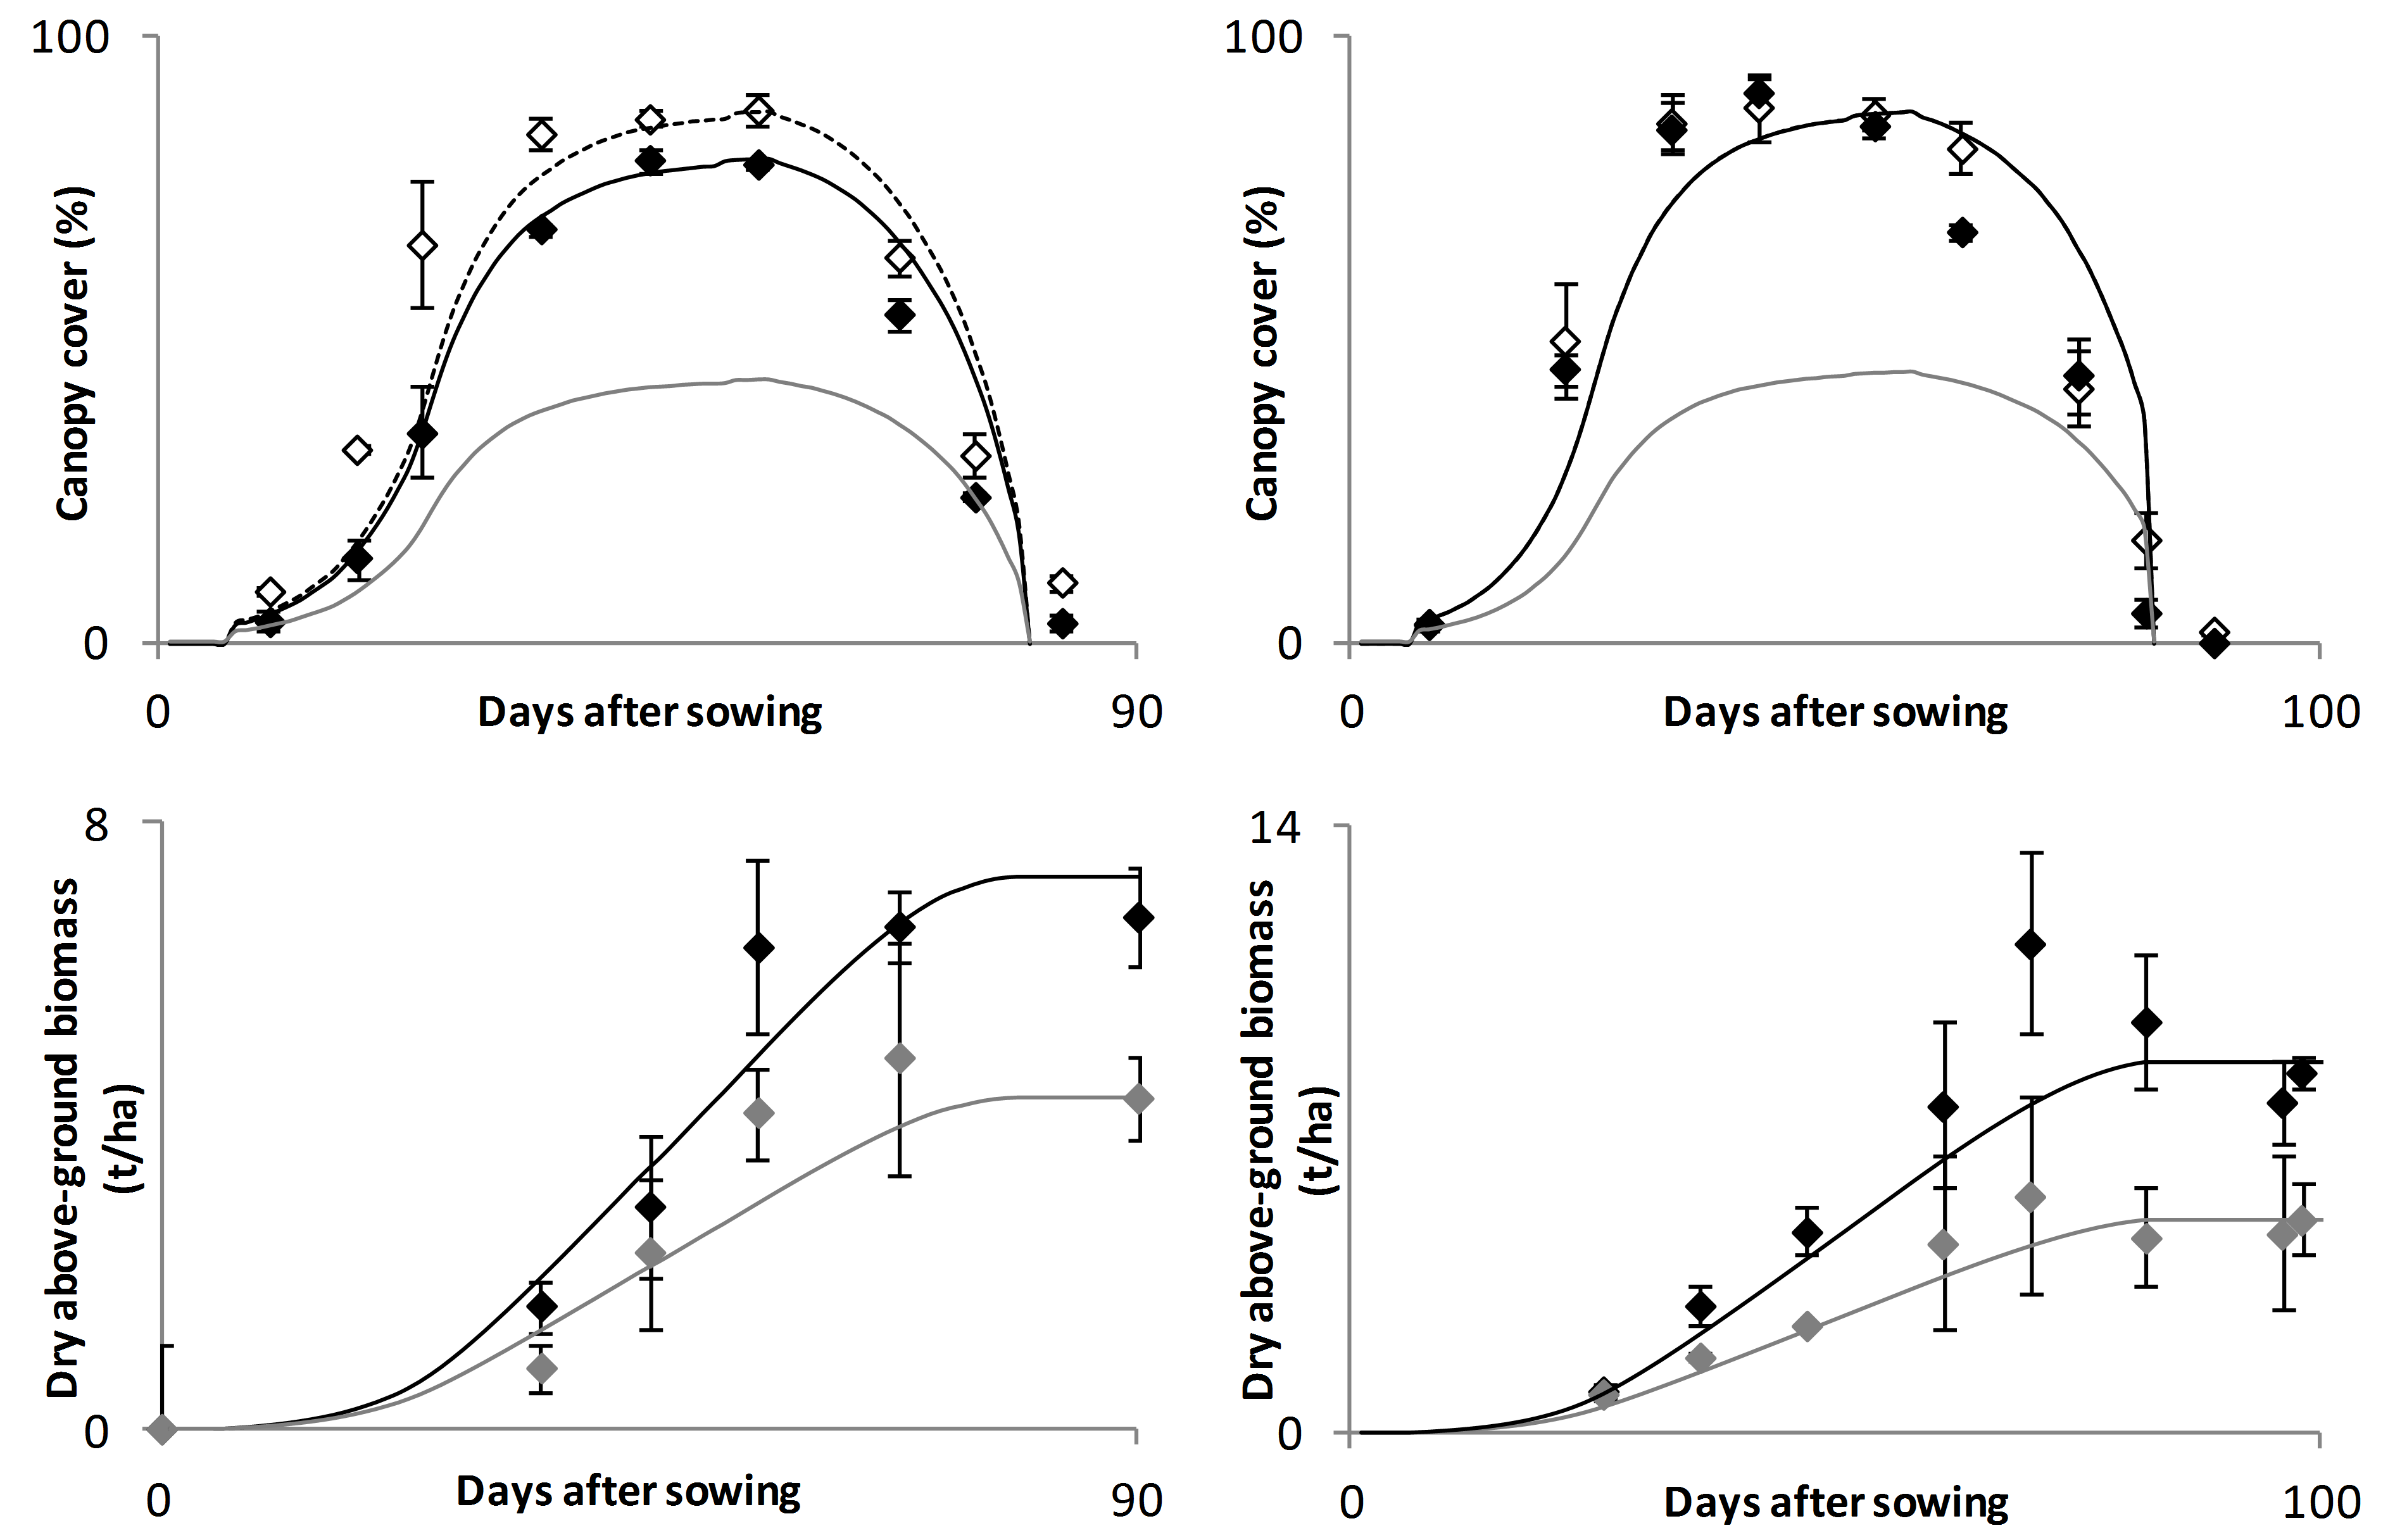
\includegraphics[width=12cm]{Barley_600dpi.png}
	\caption{Simulated (lines) and observed (symbols) canopy cover (top) and dry above-ground biomass (bottom) in well-watered barley plots in Dejen 2009 (left) and Mekelle 2010 (right). Crop canopy cover and biomass are affected by the weed infestation level: weed-free (black) and weed-infested with a relative weed cover of about 50\% (grey). The dashed line and open symbol present the total vegetation canopy cover in weed-infested conditions. Error bars indicate $\pm$ standard deviation for 3 replications.}
	\label{fig:ch4_barley}
\end{figure}  

\begin{table}[htbp]
  	\caption{Relative root-mean-square error (RRMSE), Nash-Sutcliffe model efficiency (EF) and coefficient of determination (\Rsq) for n number of observations of average soil water content in the root zone, crop canopy cover in weed-free conditions (\CCwf) or weed-infested conditions (\CCw), total vegetation canopy cover (\CCTOT), dry above-ground crop biomass (\B) during the growing season and at phenological maturity, and crop yield in weed-free and weed-infested barley and wheat plots (all experimental sites and water treatments included). Dashes indicate that observations for performance assessment were unavailable.}
    %\resizebox{\textwidth}{!}
		%{
\begin{tabular}{lcccccccc}
\toprule
       & \multicolumn{4}{c}{\textbf{Weed free}} & \multicolumn{4}{c}{\textbf{Weed infested}} \\
 & n & RRMSE& EF & \Rsq & n& RRMSE& EF & \Rsq\\
  & (-) & (\%)& (-) & (-) & (-)& (\%)& (-) & (-)\\
\midrule
Barley & & & & & & & & \\
SWCr & 33    & 11.6  & 0.80  & 0.82  & 66    & 13.2  & 0.77  & 0.78 \\
\CCwf & 36    & 22.8  & 0.90  & 0.90  &  -    &  -    &  -    &  - \\
\CCTOT &  -    &  -    &  -    &  -    & 73    & 22.3  & 0.90  & 0.90 \\
\B season & 26    & 21.2  & 0.85  & 0.88  & 52    & 23.7  & 0.83  & 0.87 \\
\B at maturity & 4     & 6.5   & 0.87  & 0.90  & 8     & 5.3   & 0.95  & 0.95 \\
Yield & 4     & 11.5  & 0.67  & 0.88  & 8     & 25.3  & 0.18  & 0.85 \\
\midrule
Wheat & & & & & & & & \\
SWCr & 32    & 4.5   & 0.68  & 0.77  &  -    &  -    &  -    &  - \\
\CCwf or \CCw & 15    & 18.1  & 0.95  & 0.96  & 15    & 14.8  & 0.96  & 0.96 \\
\CCTOT &  -    &  -    &  -    &  -    & 15    & 20.7  & 0.92  & 0.93 \\
\B season & 17    & 29.9  & 0.92  & 0.95  & 17    & 38.9  & 0.85  & 0.92 \\
\bottomrule
\end{tabular}%
%}
  \label{tab:ch4_stats}%
\end{table}

	
AquaCrop made fair predictions of barley canopy cover development and biomass build up during the growing season, as shown by the RRMSE values of between 21 to 24\% (\autoref{tab:ch4_stats}). Regardless of the fair biomass predictions during the growing season, biomass at maturity was the most accurately predicted crop variable for both weed treatments (RRMSE values of 5-6 \%). Moreover, AquaCrop made very good predictions of soil water content in the root zone (RRMSE of about 12-13\%), despite only fair predictions of canopy cover and consequently transpiration. Furthermore, \autoref{tab:ch4_stats} illustrates that simulations were slightly less accurate for weed-infested barley plots compared to weed-free conditions. RRMSE values of weed-infested treatments were only 1.5-2.5\% higher than weed-free treatments for soil water content and biomass. Predictions of barley biomass at maturity were even better than for weed-free conditions. Although final biomass was predicted excellent for all weed treatments, model performance decreased for grain yield depending on the weed treatment; barley yield predictions were very good for weed-free conditions (RRMSE of 12\%), but only fair for weed-infested conditions (RRMSE of 25\%). \autoref{fig:ch4_prod} shows that yield was overestimated for all weed treatments, while biomass was predicted accurately. This indicates overestimation of the harvest index.
 
\begin{figure}[tbhp]
	\centering
		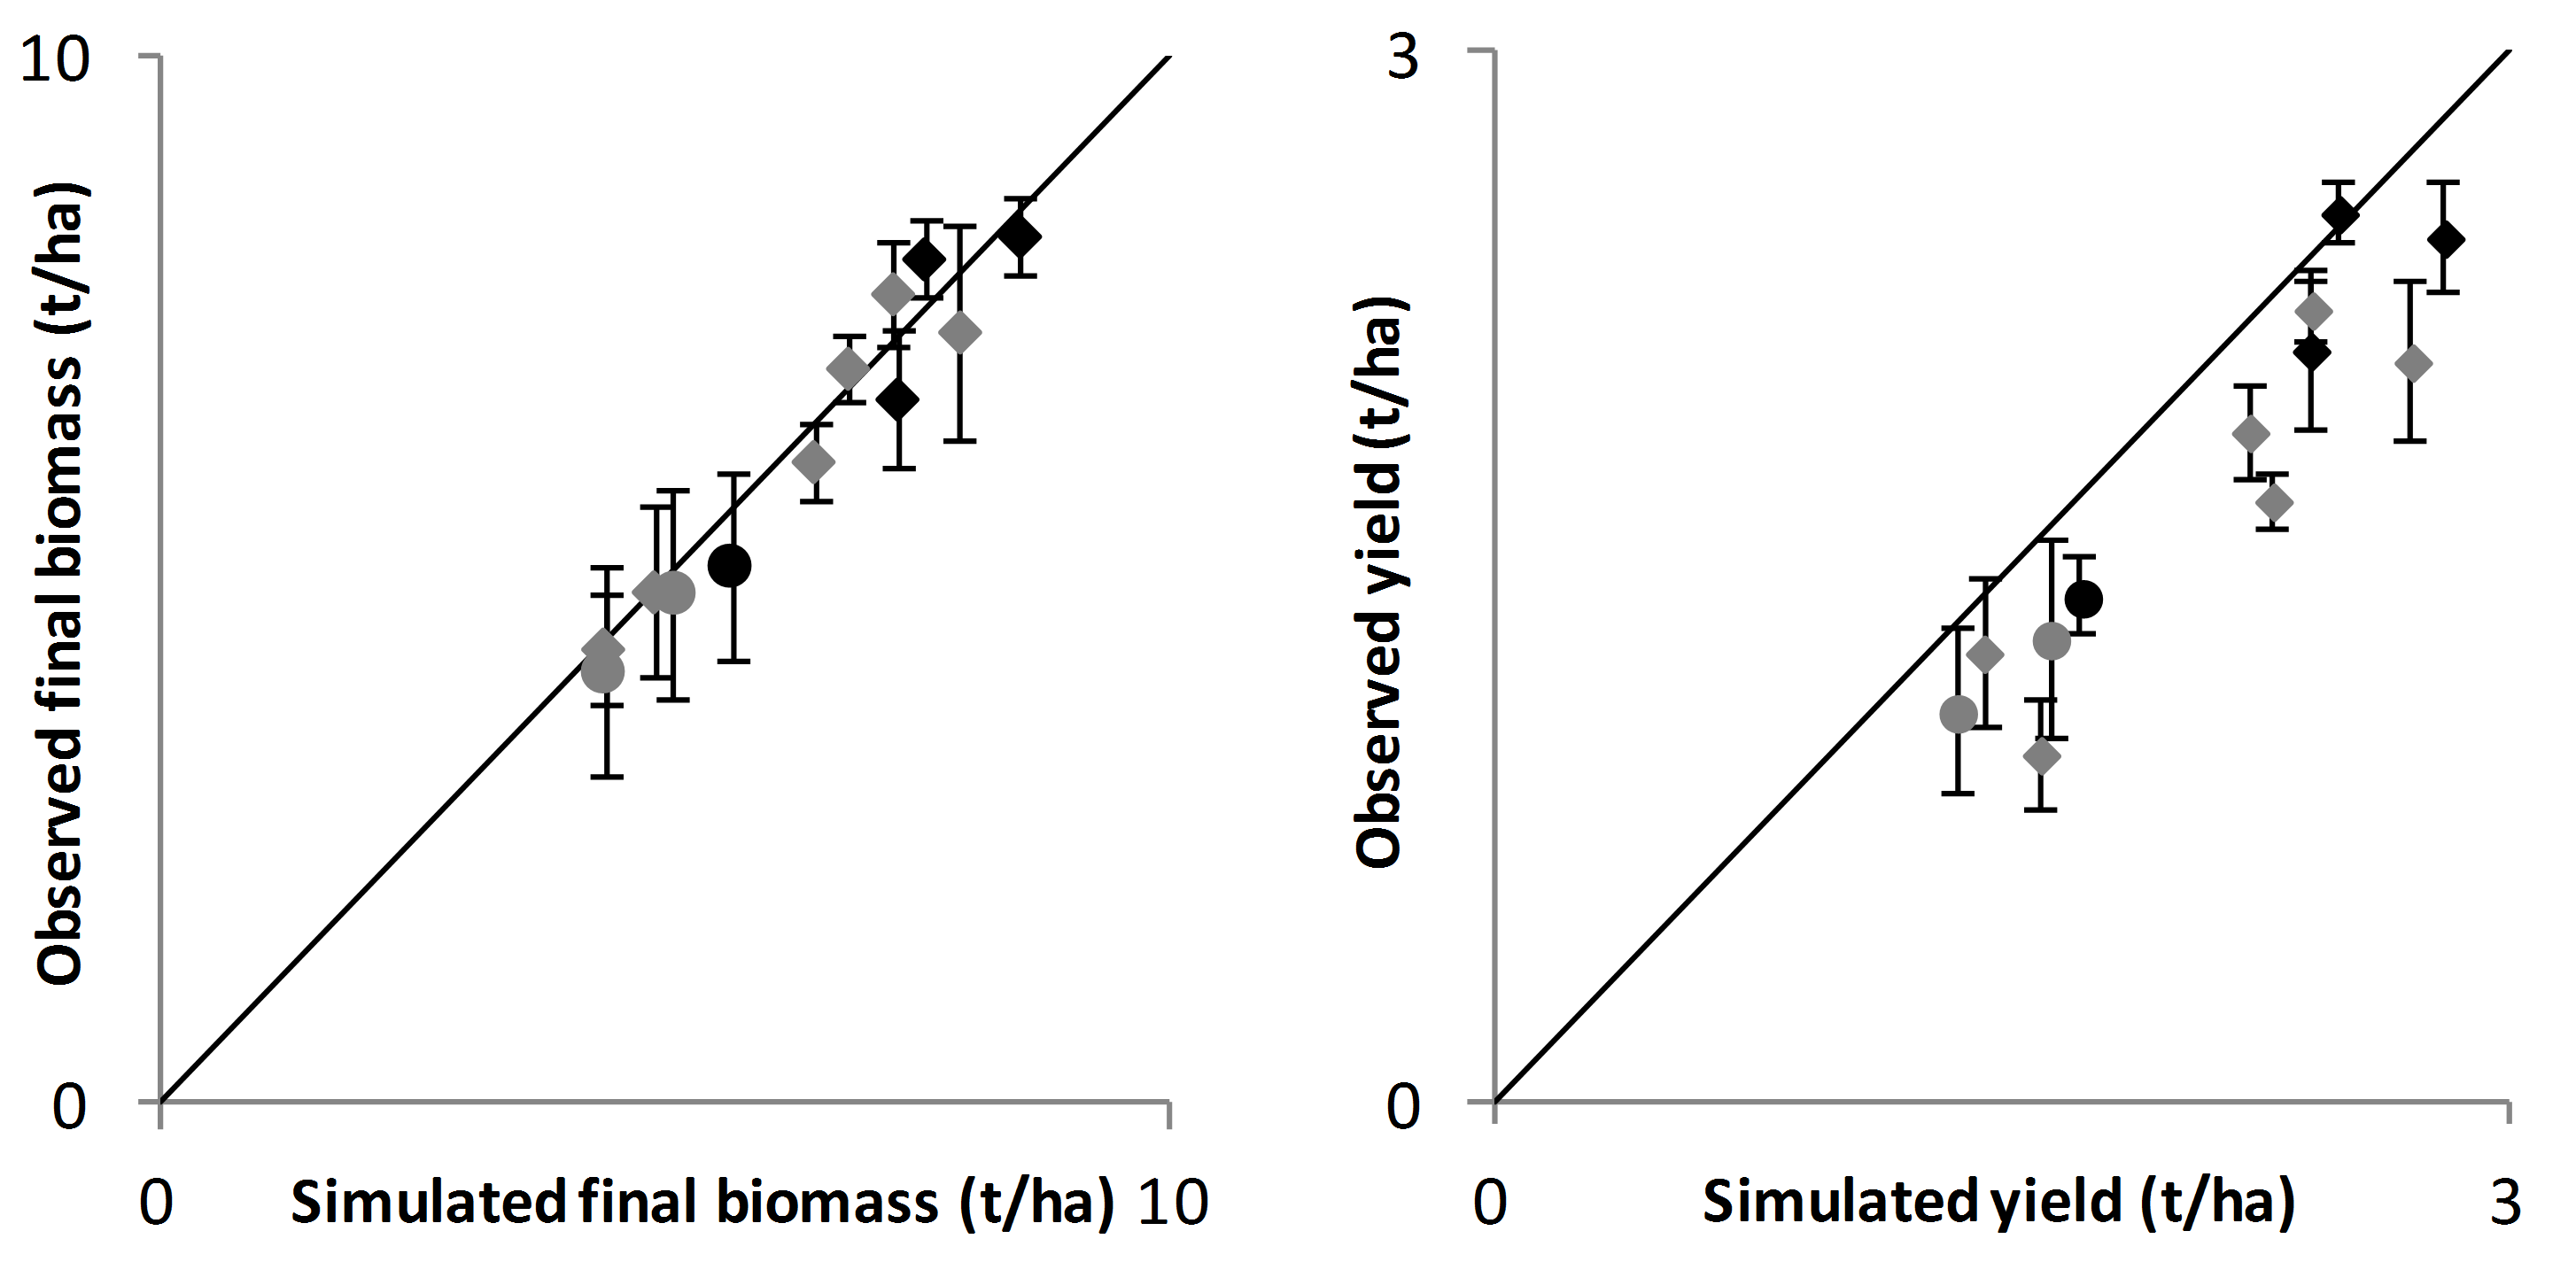
\includegraphics[]{Prod_600dpi.png}
	\caption{Observed versus simulated dry above-ground biomass at maturity (left) and grain yield (right) of barley grown in weed-free (black) and weed-infested (grey) plots with water stress (circle) or without water stress (diamond) at the three experimental sites in 2009 and 2010. Error bars indicate $\pm$ standard deviation for three replications.}
	\label{fig:ch4_prod}
\end{figure}   
 
Simulation of the soil water content in the root zone of weed-free wheat plots was excellent, as indicated by the small RRMSE value of 4.5\% (\autoref{tab:ch4_stats}). However, because soil water content simulations were less good for the S0 treatment, EF and \Rsq values were rather low. Unfortunately, observations of soil water content were not available for weed-infested fields. Furthermore, AquaCrop performed good for simulations of crop and total vegetation canopy cover, with RRMSE values between 15 and 21\%. In contrast, performance was poor for simulation of crop biomass during the season. \autoref{fig:ch4_wheat} illustrates that AquaCrop was not able to capture the slow biomass build-up during winter, even though conservative crop parameters were altered to match the characteristics of winter wheat (\autoref{tab:ch4_croppar}). Introduction of weeds further decreased model performance. In weed-infested conditions, RRMSE values were 3-9\% higher than in weed-free conditions. In spite of AquaCrop's limitations to accurately simulate biomass development, biomass at maturity was predicted very accurately with relative model errors as small as 1 to -2\%. For both water treatments, final biomass in weed-free plots was underestimated, but overestimated for weed-infested plots.
 
\begin{figure}[tbhp]
	\centering
		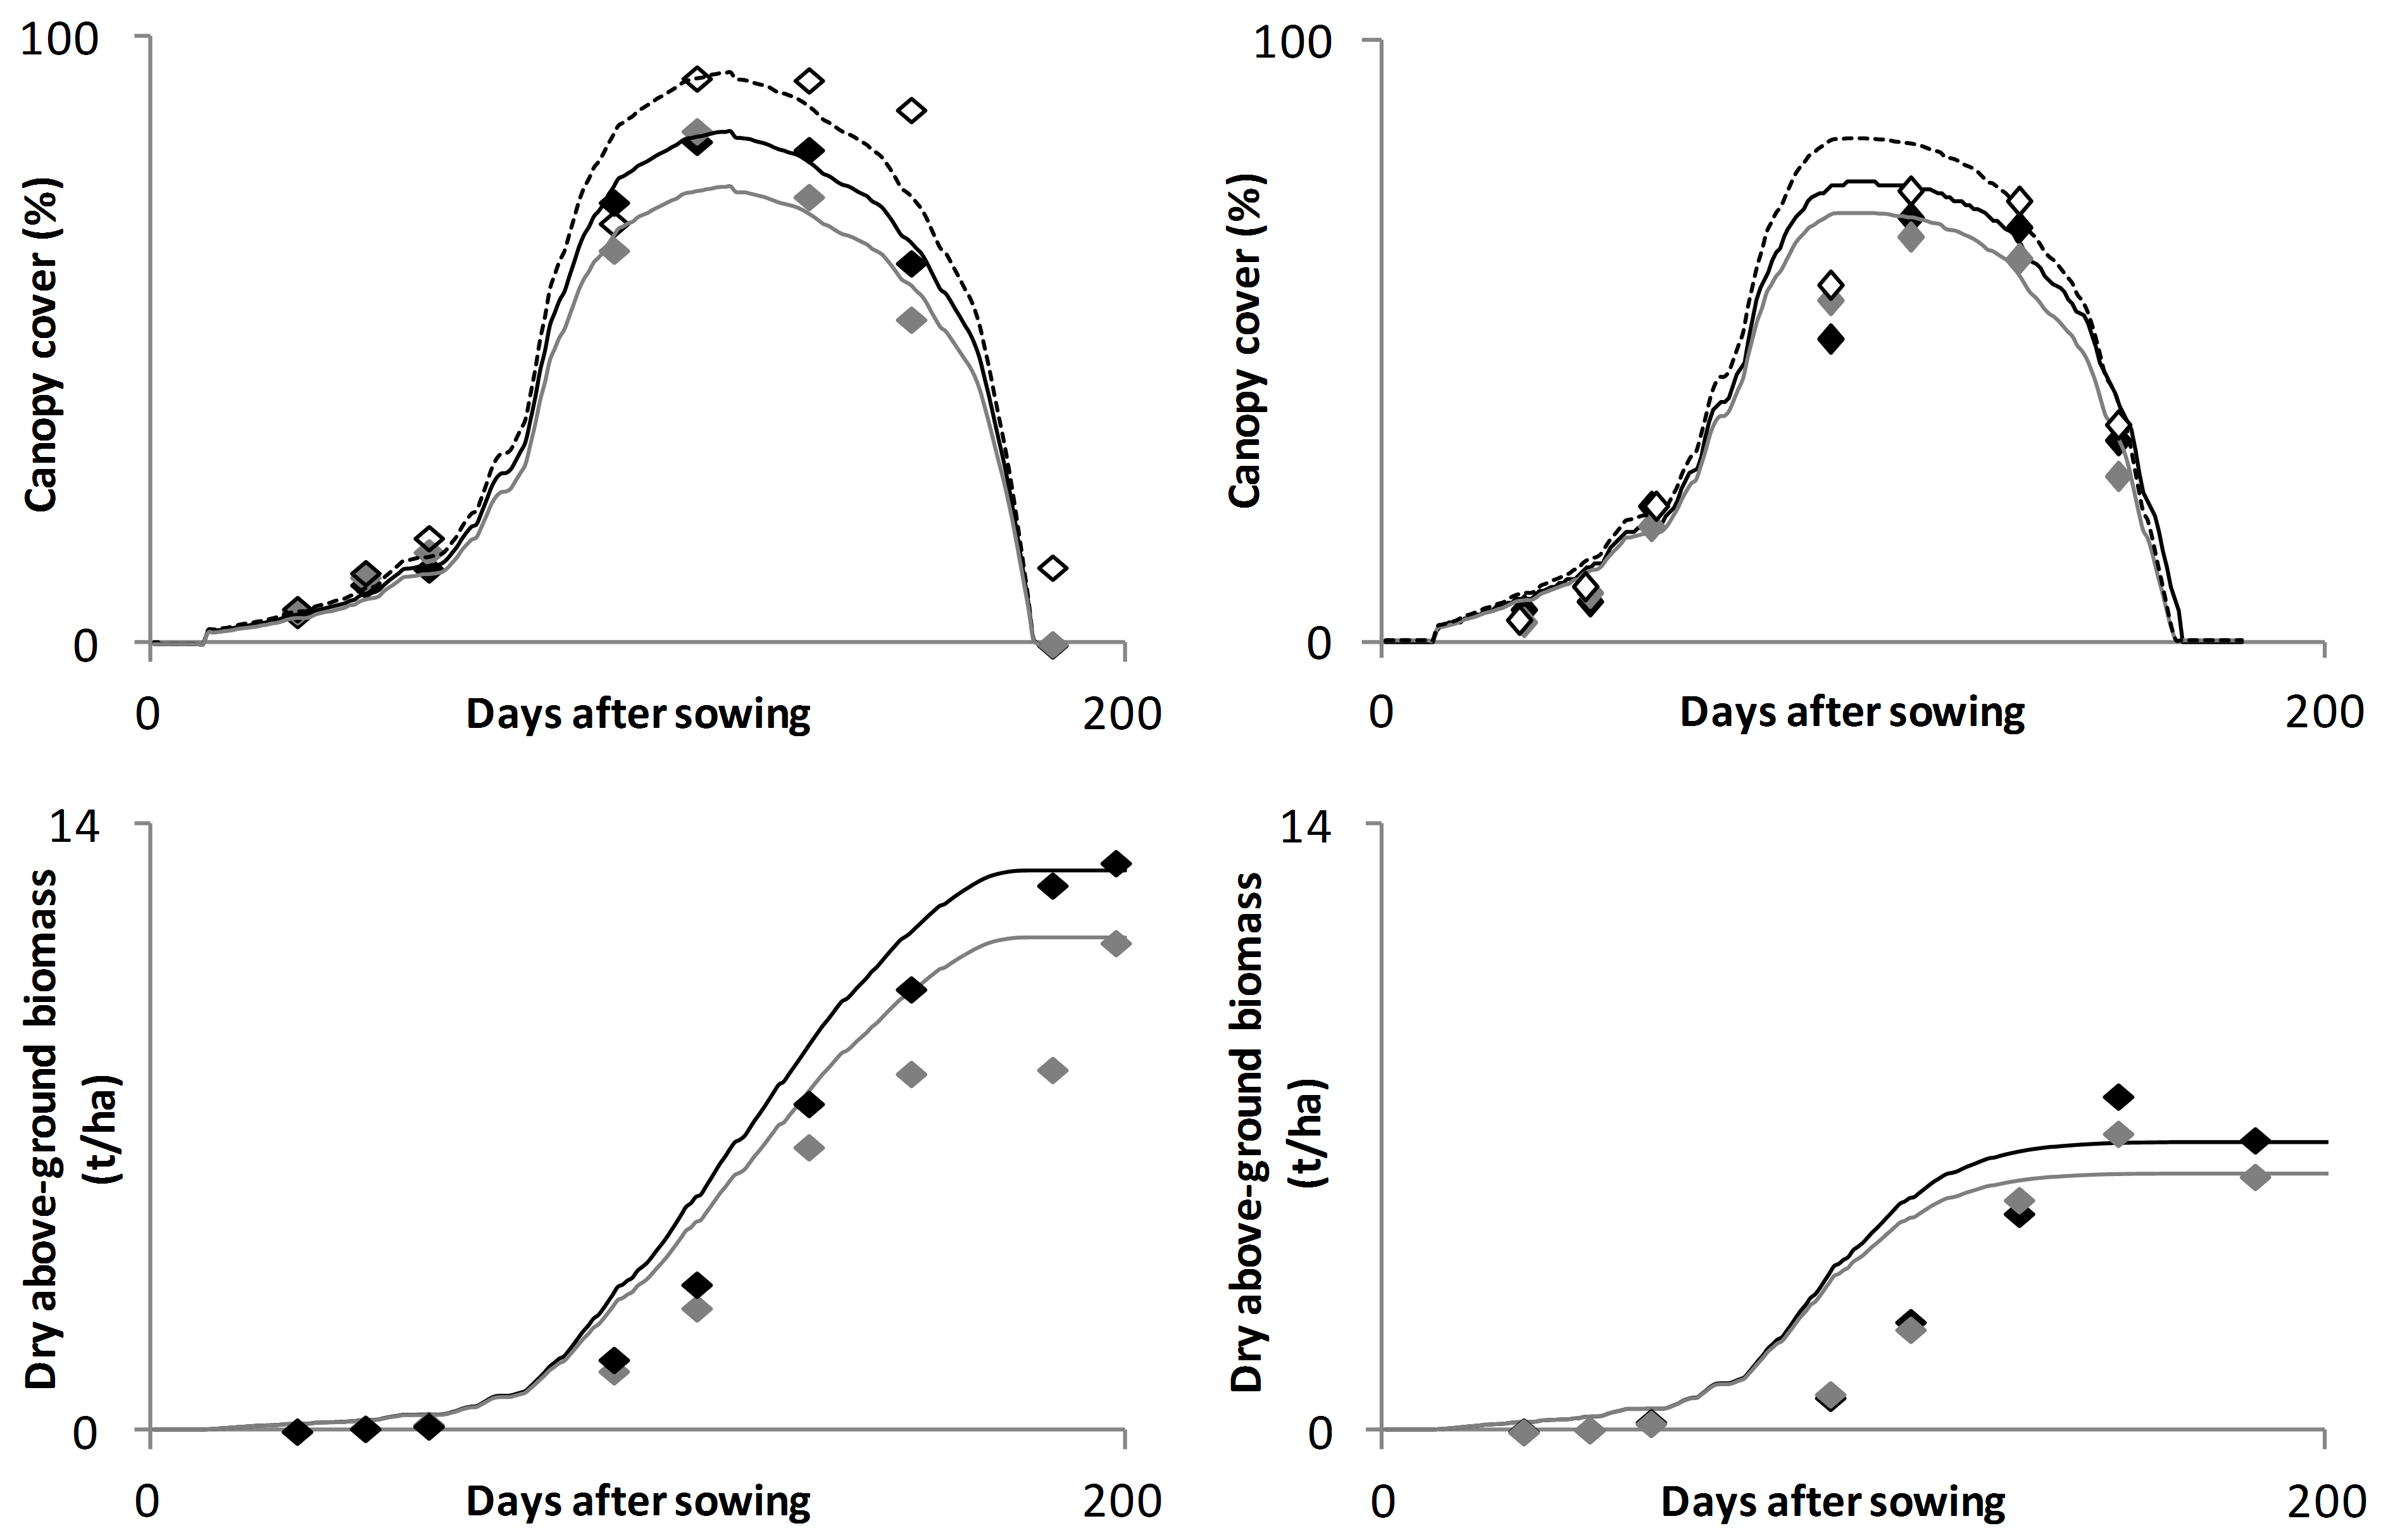
\includegraphics[width=12cm]{Wheat_600dpi.png}
	\caption{ Simulated (lines) and observed (symbols) canopy cover (top) and dry above-ground biomass (bottom) in well-watered (left) and water-stressed (right) wheat plots in Wagga Wagga, 1998. Crop canopy cover and biomass are affected by the weed infestation level: weed-free (black) and weed-infested (grey) with a relative weed cover of about 20\% for well- watered and 15\% for water-stressed plots. The dashed line and open symbol present the total vegetation canopy cover in weed-infested conditions. Data points represent an average value over five replications. Error bars indicating the standard deviation were not available for the wheat dataset.}
	\label{fig:ch4_wheat}
\end{figure}   


\section{Discussion}
\subsection{Model approach}
Data availability is a major bottleneck for application of existing crop-weed competition models. In contrast, AquaCrop requires very few input variables and parameters that can  be easily obtained. Simulation for weed-infested conditions requires only two additional inputs (\RC and \fweed), which can be easily determined by analysing digital photographs or from remote sensing images \parencite{lotz1994, burgosartizzu2009}. If such digital images are not available, one can also rely on visual estimates done in the field \parencite{andujar2010}. Since the two weed management inputs need to be specified for the weed mixture, knowledge of the exact weed species is not required. Moreover, this multiple-species approach is an important advantage, because competition by a single weed species is rarely encountered in farmers' fields.

AquaCrop  relies completely on the input of relative weed cover to simulate partitioning of resources between crop and weeds. Light partitioning is by definition represented by \RC. Water partitioning requires the total transpiration be divided into crop and weed transpiration based on total vegetation canopy cover and crop canopy cover. Since the latter are related through \RC, partitioning of water is clearly determined by \RC. Also, nutrient partitioning requires the soil fertility stress level to be adapted based on \RC. One could argue that such an \RC based approach neglects the competitive ability of weeds versus crop to obtain light, water and nutrients. Also, differences in sensitivity to scarcity of these resources seem to be neglected. However, this is not true since \fweed incorporates the competitive ability of crop and weed to obtain light. In addition, \RC serves as a proxy for competitive ability and sensitivity to water and soil fertility stress. Also, \textcite{aldrich1987} found light competition to be representative for total competition, since canopy size and structure is the result of competition for light, water and nutrients, as well as allelopathic interactions. Moreover, photosynthesis is not just involved in light competition, but also provides the energy for uptake of nutrients and water. 

Furthermore, AquaCrop uses a static approach regarding weed infestation, as it uses a constant value of \RC at time of maximum canopy cover to define the effect of weeds on crop canopy cover during the whole growing season. Such a static approach neglects the dynamics of weed cover, which can increase or decrease during the growing season depending on the competitive ability of crop versus weed. However, the absolute error made with this static approach is negligible at the beginning of the growing season, because canopy cover is still very small and little biomass is produced during the canopy expansion phase. In contrast, the error could be larger in mid-season, when crop canopy cover is large and most biomass is produced. Although the current study proved that good model results can be obtained with the static approach, future research should indicate whether \RC dynamics in mid-season have a large impact on model results, and should be incorporated in the model.    
 
Finally, it should be noted that AquaCrop's representation of the crop-weed vegetation as a single theoretical crop with the same growing cycle as the weed-free crop neglects possible differences between the crops' and weeds' growing cycles. Nevertheless, this simplification is valid both for late-emerging weeds, that cannot outgrow the crop, and for early-emerging weeds, which are removed during land preparation. Moreover, weeds with a life cycle similar to that of the crop will usually be the most successful competitors \parencite{zimdahl2013} and consequently lead to major yield losses.

\subsection{Model performance}
AquaCrop performed well for simulated barley growth and production. This indicates that the selected crop parameters and inputs were a good representation of the local environment and cropping system. As the default crop parameters had been calibrated and validated by \textcite{abrha2012} for the same local barley variety grown in weed-free conditions, this is no surprise. Overestimation of yield indicated incorrect simulation of the harvest index, especially in weed-infested plots. This could be due to inaccurate settings of the barley water stress thresholds, or because AquaCrop disregards any direct effect of weeds on grain formation. Field experiments show that weeds can reduce barley grain yield by lowering the number of ear bearing tillers, number of grains per ear, and 1000-kernel weight \parencite{wilson1982, morishita1988}. Introducing an \RC-dependent stress coefficient that affects the harvest index, could improve model simulations. However, this would also lead to extra parameter uncertainty in the model. 

Model performance to simulate wheat production was less good compared to barley, in particular for simulation of biomass during the growing season. It is expected that introduction of an extra stress coefficient to represent slow crop development because of low winter temperatures, as previously proposed by \textcite{vanuytrecht2013}, would significantly improve AquaCrop's performance for both weed-free and weed-infested winter wheat simulations. Despite the poor in-season biomass predictions, AquaCrop made excellent predictions of wheat biomass at maturity. In practice, final biomass, and not intermediate biomass, is most crucial to assess weed-induced yield losses. 

Moreover, AquaCrop's performance for the wheat dataset was well within the performance range of four mechanistic crop-weed competition models (ALMANAC, APSIM, CROPSIM, INTERCOM) that were tested with the same dataset by \textcite{deen2003}(Box \ref{box:ch4_compare}). However, this model performance comparison should be interpreted with care, as the AquaCrop approach is very different from mechanistic crop-weed competition models. The latter predict both crop and weed growth, partitioning of resources between crop and weed, and the resulting crop yield loss due to weeds. AquaCrop, on the other hand, uses input of the observed effect of weeds on crop canopy cover at time of canopy closure to simulate the effect of weeds on the soil water balance and crop production.

Finally, it should be noted that because of the experimental setup, the current study  focused mainly on simulation of the outcome of crop-weed competition for light. Model performance for water competition was assessed based on the weed-infested, water-stressed treatments, which were only available for one of the barley experiments (Maiquiha 2009) and the wheat experiment. Although model performance proved very promising for these experiments, additional research including different water stress levels, ranging between low and very severe water stress, could further reveal to what extent AquaCrop can accurately capture the effect of weeds on soil water content and crop water availability. Furthermore, competition for nutrients was not considered in this study, because the soil fertility level was optimal in all experiments. Therefore, further evaluation of AquaCrop for weed-infested, soil-fertility-stressed fields remains necessary. 

\newtcolorbox[auto counter,number within=chapter]{MyBox2}[1][]{
  enhanced,
  breakable,
  %float,
  parbox=false, % zodat de paragrafen zijn zoals in de text
  title=Box \thetcbcounter : Model comparison for simulation of weed-infested wheat fields,
  #1} % dit is voor het label te fixen

\begin{MyBox2}[label = box:ch4_compare]

AquaCrop's performance to simulate wheat production for the experiment in Wagga Wagga (1998) was compared with the performance of ALMANAC, APSIM, CROPSIM and INTERCOM as reported by \textcite{deen2003}. Simulated LAI values were converted to CC values using \autoref{eq:ch4_LAIconvert} to enable model comparison. Models were compared based on the calculated RRMSE or RME in case of low number of observations. 

In spite of AquaCrop’s limitations to accurately simulate wheat development during winter, \autoref{fig:ch4_compareCCB} shows that AquaCrop’s performance to simulate crop canopy cover and biomass development was within the performance range of ALMANAC, APSIM, CROPSIM and INTERCOM. The five models covered a wide range from excellent to very poor performance, with RRMSE values of about 5 to 60\%. AquaCrop simulations of crop canopy cover were most accurate of all models, apart from simulations for weed-free, water stressed conditions for which AquaCrop performed second best. In contrast, AquaCrop's performance was amongst the poorest for simulation of biomass during the season. Particularly in water-stressed conditions, RRMSE values revealed very poor model performance. Nevertheless, APSIM, CROPSIM, and INTERCOM performed even worse for some water or weed treatments.

\begin{center}
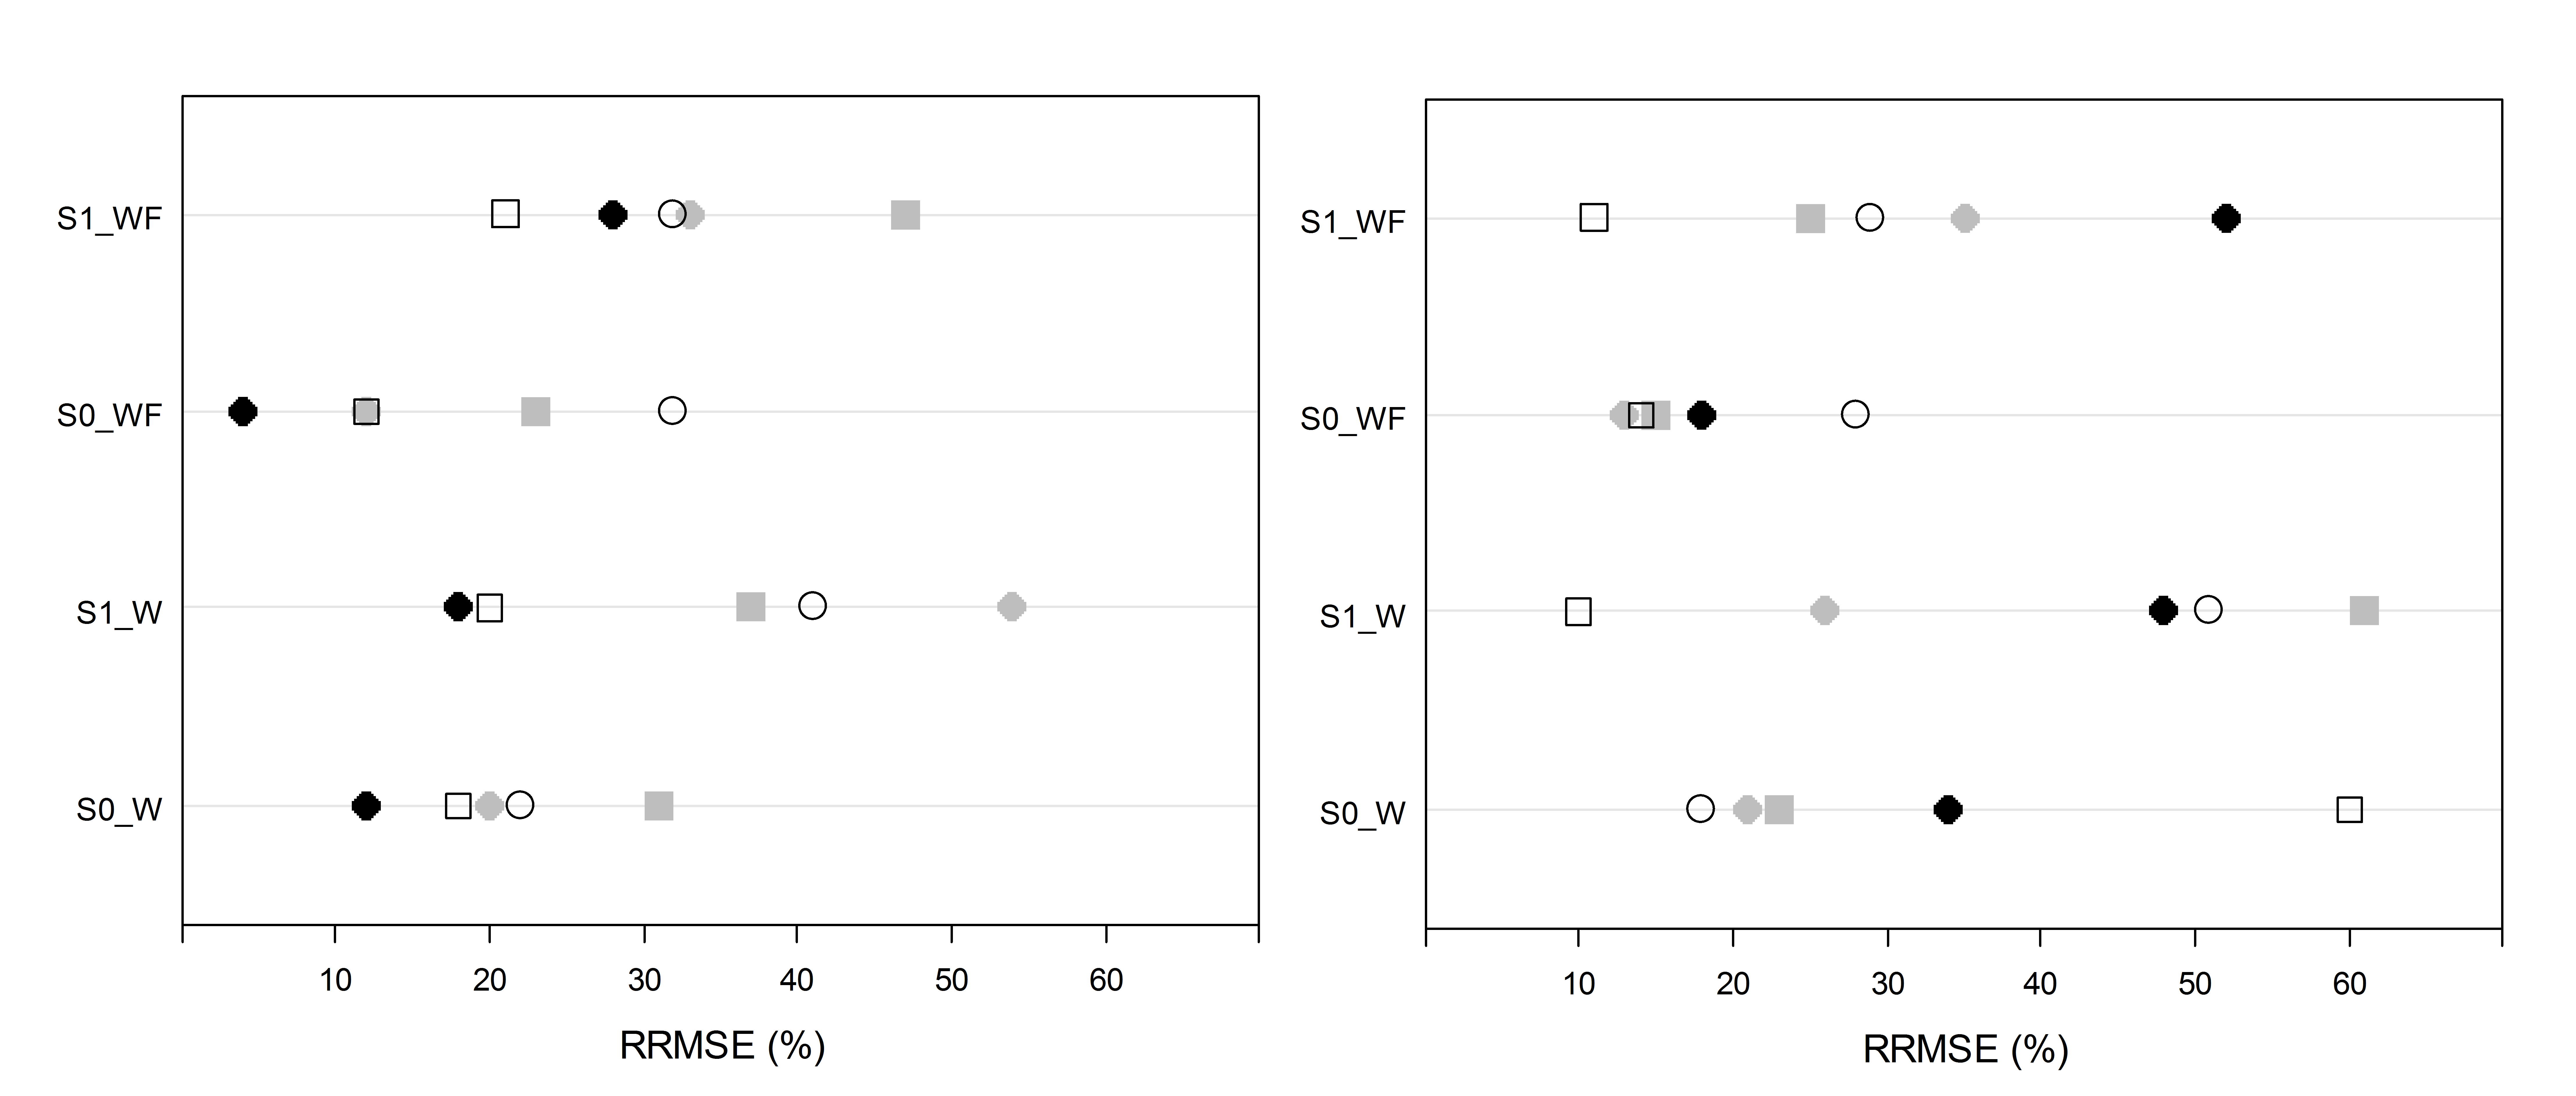
\includegraphics[width=\textwidth]{CompareCCB_600dpi.png}
\end{center}
\label{fig:ch4_compareCCB}
\captionof{figure}{The relative root-mean-square error (RRMSE) for wheat canopy cover (left) and biomass during the growing season (right) varies between different models: AquaCrop ($\bullet$), ALMANAC (\textcolor{gray}{$\bullet$}), APSIM($\circ$), CROPSIM (\textcolor{gray}{$\blacksquare$}) and INTERCOM($\square$). Model performance also differs between water and weed treatments: absence (S0) or presence (S1) of water stress, weed-free (WF) or weed-infested (W).}
\bigskip
Although biomass during the season was predicted rather poor, final biomass deviation (RME) was maximum 2\% for AquaCrop (\autoref{fig:ch4_compareCCB}). With these small deviations, AquaCrop was superior to all other models that had RME values as big as 27\% or -25\%. While the other models systematically overestimated (ALMANAC and INTERCOM) or underestimated (CROPSIM and APSIM) final biomass, AquaCrop did not show systematic deviation. Final biomass at maturity was slightly overestimated in weed-infested conditions, but underestimated in weed-free plots. 

\begin{center}
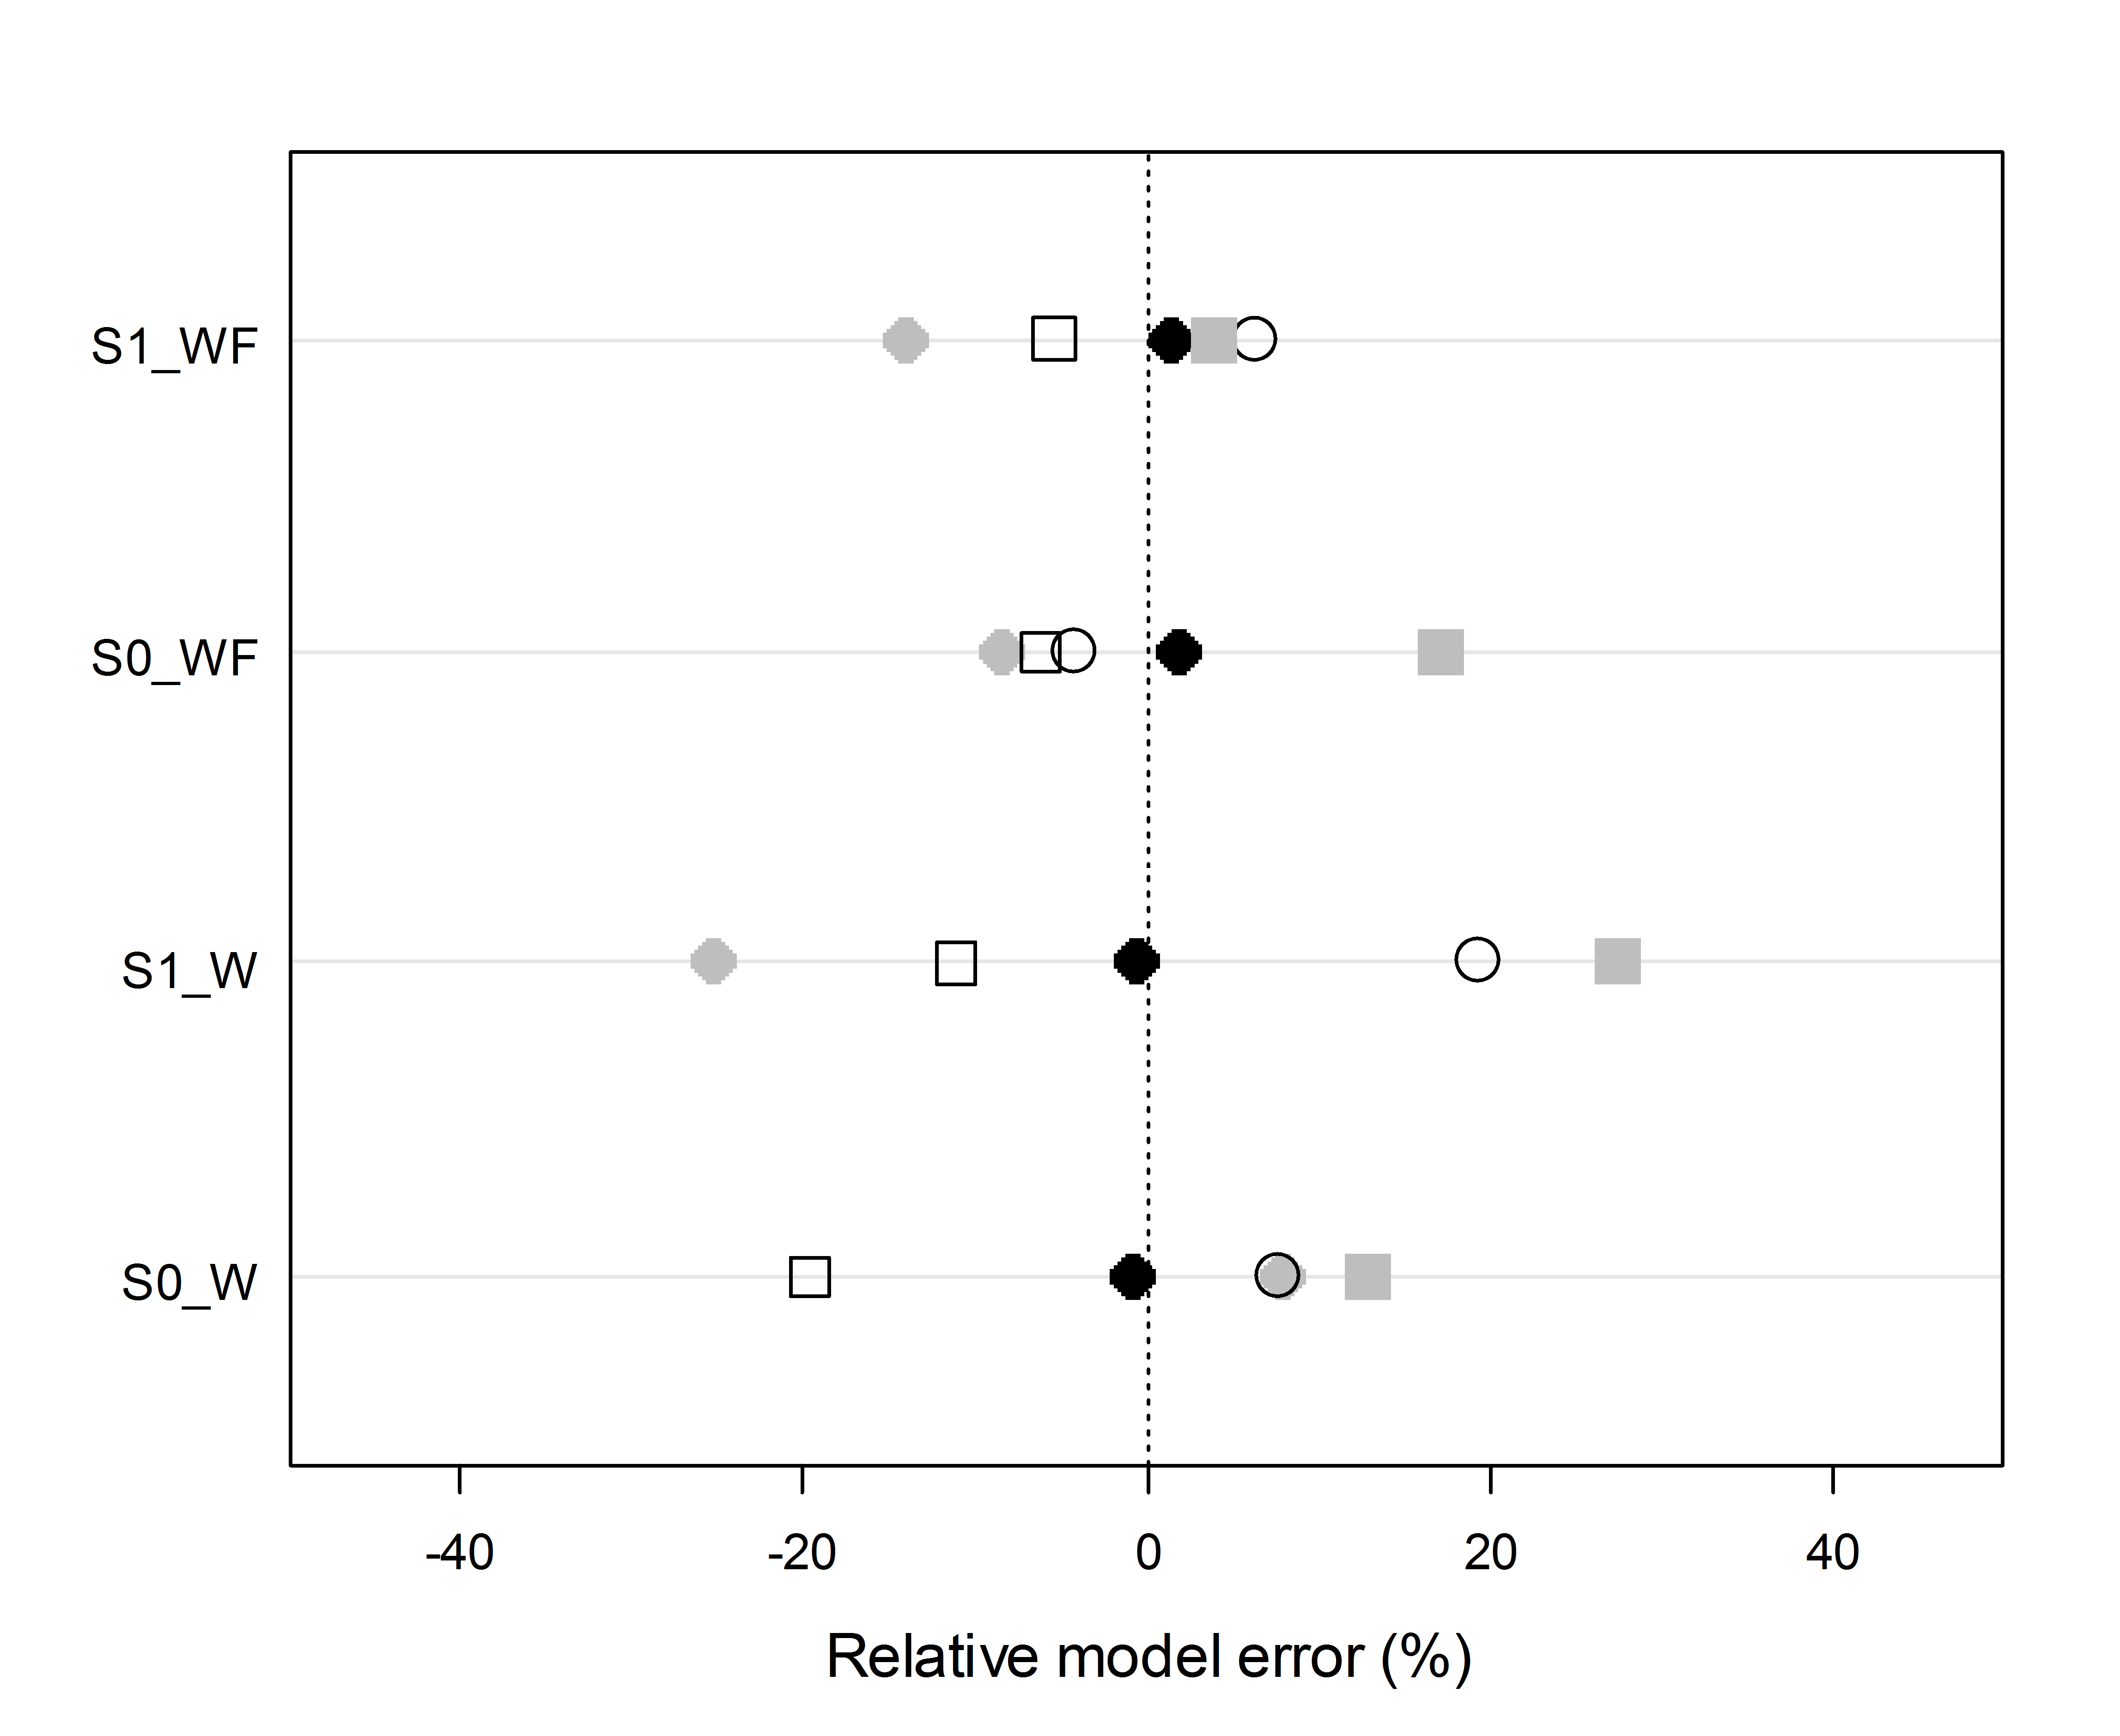
\includegraphics[width=7cm]{CompareB_600dpi}
\end{center}
\label{fig:ch4_comparefinalB}
\captionof{figure}{Deviation between simulated and observed biomass at maturity varies between different models: AquaCrop ($\bullet$), ALMANAC (\textcolor{gray}{$\bullet$}), APSIM($\circ$), CROPSIM (\textcolor{gray}{$\blacksquare$}) and INTERCOM($\square$). Model deviation also differs between water and weed treatments: absence (S0) or presence (S1) of water stress, weed-free (WF) or weed-infested (W).}

\end{MyBox2}

\subsection{Model application} 
Once properly calibrated to the local environment and cropping system, AquaCrop can be used to simulate crop growth, production and water productivity in weed-infested fields. Notwithstanding its simple approach, the new weed module is widely applicable. This was demonstrated by model evaluation for various experimental setups including different locations, soil types, climatic conditions, water treatments, crops, weed species and weed infestation levels. Furthermore, limited input and calibration requirements make AquaCrop applicable in data-scarce regions. If data are sparse, weed management inputs can even be specified in qualitative terms. A user can select one of the predefined \RC classes, ranging between `very poor' and `perfect' weed management, or one of the predefined \fweed classes ranging between `very weak' and `very strong' weed-induced increase of total canopy cover. In addition, the transparent simulation procedure and user-friendly interface enable application by non-specialists.

Addition of weed infestation as a production- and water-limiting factor improves accuracy of yield predictions and yield gap analysis in weed-infested areas. Other potential model applications include investigation of tolerable weed infestation levels, as well as assessment of yield loss mitigation strategies such as changing sowing density or crop type. AquaCrop has the important advantage that weed infestation scenarios can be evaluated based on both simulated crop yield and crop water productivity. Assessing both these productivity indicators is vital in water scarce regions, where management decisions should be made in view of limited water availability. 

Even though potential applications are numerous, the AquaCrop approach has limitations. The model can only support strategic management decisions, and cannot be used for assessment of tactical decisions. For example, model simulations can provide information on tolerable weed infestation levels, but can optimize neither pesticide dose nor timing of weed control operations. Moreover, the model cannot provide additional insights into the competition mechanisms. This would require a more detailed, process-based approach as adopted by other mechanistic models. Finally, it is clear that AquaCrop can support weed management decisions only from an agronomic point of view. However, by linking AquaCrop to an economic model, weed management can be optimized accounting for factors including labour and time requirement of weed control operations, prices of herbicides and prices of crop products. An example was set by \textcite{dunan1994, dunan1999} who optimized weed management based on both agronomic and economic aspects. Moreover, the linkage of AquaCrop to economic models has been demonstrated by \textcite{garciavila2009}, \textcite{garciavila2012} and \textcite{cusicanqui2013}.

\section{Conclusions}
The AquaCrop approach to simulate crop production in weed-infested fields proves to be a very intuitive approach that requires just two easily obtainable input variables: the relative leaf cover of weeds and weed-induced increase of total canopy cover. This makes the model applicable to all herbaceous crops grown in competition with any type or number of weeds. Despite its simple approach, AquaCrop performs good to simulate soil water content, crop development and crop production in weed-infested barley and wheat fields over a wide range of environmental and agronomic conditions. Further testing of the model remains necessary to assess model performance for weed-infested conditions combined with nutrient limitations or severe water stress. Because of its simple but accurate simulation procedure, wide applicability and low data requirements, AquaCrop is a practical tool to investigate the effect of weed infestation on crop production in data-scarce regions. 


\cleardoublepage